%% Copernicus Publications Manuscript Preparation Template for LaTeX Submissions
%% ---------------------------------
%% This template should be used for copernicus.cls
%% The class file and some style files are bundled in the Copernicus Latex Package, which can be downloaded from the different journal webpages.
%% For further assistance please contact Copernicus Publications at: production@copernicus.org
%% https://publications.copernicus.org/for_authors/manuscript_preparation.html


%% Please use the following documentclass and journal abbreviations for preprints and final revised papers.

%% 2-column papers and preprints
\documentclass[gmd, manuscript]{copernicus}



%% Journal abbreviations (please use the same for preprints and final revised papers)


% Advances in Geosciences (adgeo)
% Advances in Radio Science (ars)
% Advances in Science and Research (asr)
% Advances in Statistical Climatology, Meteorology and Oceanography (ascmo)
% Annales Geophysicae (angeo)
% Archives Animal Breeding (aab)
% ASTRA Proceedings (ap)
% Atmospheric Chemistry and Physics (acp)
% Atmospheric Measurement Techniques (amt)
% Biogeosciences (bg)
% Climate of the Past (cp)
% DEUQUA Special Publications (deuquasp)
% Drinking Water Engineering and Science (dwes)
% Earth Surface Dynamics (esurf)
% Earth System Dynamics (esd)
% Earth System Science Data (essd)
% E&G Quaternary Science Journal (egqsj)
% European Journal of Mineralogy (ejm)
% Fossil Record (fr)
% Geochronology (gchron)
% Geographica Helvetica (gh)
% Geoscience Communication (gc)
% Geoscientific Instrumentation, Methods and Data Systems (gi)
% Geoscientific Model Development (gmd)
% History of Geo- and Space Sciences (hgss)
% Hydrology and Earth System Sciences (hess)
% Journal of Bone and Joint Infection (jbji)
% Journal of Micropalaeontology (jm)
% Journal of Sensors and Sensor Systems (jsss)
% Magnetic Resonance (mr)
% Mechanical Sciences (ms)
% Natural Hazards and Earth System Sciences (nhess)
% Nonlinear Processes in Geophysics (npg)
% Ocean Science (os)
% Polarforschung - Journal of the German Society for Polar Research (polf)
% Primate Biology (pb)
% Proceedings of the International Association of Hydrological Sciences (piahs)
% Scientific Drilling (sd)
% SOIL (soil)
% Solid Earth (se)
% The Cryosphere (tc)
% Weather and Climate Dynamics (wcd)
% Web Ecology (we)
% Wind Energy Science (wes)


%% \usepackage commands included in the copernicus.cls:
%\usepackage[german, english]{babel}
%\usepackage{tabularx}
%\usepackage{cancel}
%\usepackage{multirow}
%\usepackage{supertabular}
%\usepackage{algorithmic}
%\usepackage{algorithm}
%\usepackage{amsthm}
%\usepackage{float}
%\usepackage{subfig}
%\usepackage{rotating}


\begin{document}

\title{Constraining the carbon cycle in JULES-ES-1.0}

% \Author[affil]{given_name}{surname}

\Author[1,2]{Doug}{McNeall}
\Author[1]{Eddy}{Robertson}
\Author[1,2]{Andy}{Wiltshire}

\affil[1]{Met Office, FitzRoy Road, Exeter, EX1 3PB}
\affil[2]{College of Engineering, Mathematics, and Physical Sciences, University of Exeter, Exeter, EX4 4QE, UK}
\affil[3]{College of Life and Environmental Sciences, University of Exeter, Exeter, EX4 4RJ, UK}

%% The [] brackets identify the author with the corresponding affiliation. 1, 2, 3, etc. should be inserted.

%% If an author is deceased, please mark the respective author name(s) with a dagger, e.g. "\Author[2,$\dag$]{Anton}{Aman}", and add a further "\affil[$\dag$]{deceased, 1 July 2019}".

%% If authors contributed equally, please mark the respective author names with an asterisk, e.g. "\Author[2,*]{Anton}{Aman}" and "\Author[3,*]{Bradley}{Bman}" and add a further affiliation: "\affil[*]{These authors contributed equally to this work.}".


\correspondence{Doug McNeall (doug.mcneall@metoffice.gov.uk)}

\runningtitle{Constraining the carbon cycle in JULES-ES1.0}

\runningauthor{McNeall et al.}

\received{}
\pubdiscuss{} %% only important for two-stage journals
\revised{}
\accepted{}
\published{}

%% These dates will be inserted by Copernicus Publications during the typesetting process.


\firstpage{1}

\maketitle

\begin{abstract}

Land surface models are an important tool in the study of climate change and its impacts, but their use can be hampered by uncertainties in input parameter settings and by errors in the models. We apply Uncertainty Quantification (UQ) techniques to constrain the input parameters of JULES-ES-1.0, the land surface component of the UK Earth system model UKESM1.0. We use an ensemble of historical simulations of the land surface model to rule out ensemble members and corresponding input parameter settings that do not match modern observations of the land surface. As JULES-ES-1.0 is computationally expensive, we use a cheap statistical proxy termed an emulator, trained on the ensemble of model runs, to rule out untested parts of parameter space. We use history matching, an iterated approach to constraining JULES-ES-1.0, running an initial ensemble and training the emulator, before choosing a second wave of ensemble members consistent with historical land surface observations. We rule out 88\% of the initial input parameter space as being statistically inconsistent with observed land surface behaviour. We use sensitivity analysis to identify the most (and least) important input parameters for controlling the global output of JULES-ES-1.0, and provide information on how parameters might be varied to improve the performance of the model and eliminate model biases.

\end{abstract}

\copyrightstatement{ $\copyright$ Crown copyright, Met Office} %% This section is optional and can be used for copyright transfers.

\introduction\label{sec:introduction}  %% \introduction[modified heading if necessary]

Land surface models are widely used for the study and projection of climate change and its impacts, but differences between the models and the systems they represent can linit their effectiveness \citep{fisher2020perspectives}. These differences can be caused by fundamental errors or a lack of knowledge of real world processes, or by the simplifications and compromises required to build and run the computationally expensive computer models that we use to simulate those processes. Uncertainty quantification (UQ) methods have been developed in order to identify and quantify the differences between the models and the real world, how to minimise those differences, and how to asses their impact on the use of models in policy advice.

Complex land surface models contain a large number of tuneable input parameters - numbers which represent simplifications of processes which are either unnecessary or too computationally expensive to include in a simulation. The value of a particular input parameter can materially affect the output of a model, but it is often unclear exactly how until the corresponding simulations are run. Input parameters may represent some real-world quantity, and so a modeller may have a belief about the "correct" value of that input parameter, that they are able to represent with a probability distribution. As processes interact within a model, input parameters can rarely be tuned in isolation to each other. For many climate applications, a goal is to choose the ranges of input parameters so that the model behaves consistently with our understanding of the behaviour of the true system, and that is consistent with our knowledge of the value that those input parameters have in the real world. The input parameters of such a model are said to be "constrained", and any simulations of future behaviour will be constrained by our choice of input settings to be consistent with our best understanding of the system.

As we have uncertainty about the structure and the behaviour of the true system, through a lack of knowledge or through uncertain observations, the value of the "best" configuration of input parameters and their associated probability distributions is uncertain. In practice, modellers often use constrained ranges of input parameter to run collections of model evaluations termed "ensembles", crudely representing uncertainty about the behaviour of the true system.

Perturbed parameter ensembles (PPEs) are useful for the evaluation of complex and computationally expensive climate models, including land surface models. A PPE is a collection of simulator runs where input parameters are systematically varied in line with a set of principles consistent with our knowledge and experiment objectives. PPEs allow a quantification of the relationship between the model input parameters and its output. They can therefore be used for the quantification and propagation of uncertainty in parameter constraint, in sensitivity of the model outputs to perturbations, and can give hints as to the size and location of model structural errors.

PPEs are now standard practice in the study of climate models for uncertainty quantification, climate and impacts projection (e.g. \cite{sexton2021perturbed, edwards2019revisiting}), parameterisation improvement \citep{couvreux2021process}, sensitivity analysis \citep{carslaw2013large}, or as part of a strategy for model development and bias correction (e.g. \cite{williamson2015identifying,mcneall2016impact, mcneall2020correcting, hourdin2017art}.

The size of PPEs is often limited by the computational expense of the complex models that they are used for, and so there is a natural tension between model complexity, resolution and the length of simulations, and the number of ensemble members available for parameter uncertainty quantification. A cheap surrogate model (sometimes termed metamodel, or emulator) is useful to maximise the utility of an ensemble in these situations. Emulators are statistical models or machine learning algorithms, usually trained on a PPE that has been carefully designed to cover input space effectively. Gaussian process emulators, used in this study, have an advantage in that they are naturally flexible and natively include uncertainty estimates as to their error, but simpler linear model and more complex machine learning approaches are possible and can be effective.

\subsection{Experiment structure}\label{ssec:experiment_structure}

In this paper, we develop a comprehensive PPE of JULES-ES-1.0, and compare it with observations to ensure that its members are broadly consistent with historical behaviour of the land surface. Our focus in on global totals of carbon cycle-relevant quantities, which are of direct interest for carbon budget assessments such as the Global Carbon Budget \citep{essd-14-1917-2022}. The ensemble is designed to be a flexible basis for a number of initial analyses, and provide a foundation for further exploration in uncertainty quantification of both historical and future projections of the land surface and carbon cycle.  We would like an ensemble with members that fully represent and sample the spread of uncertainty we have in historical land surface characteristics and behaviour. We would also like an ensemble large enough to effectively train a an emulator, in order to perform a number of the analyses.

Our approach could be regarded as a "top-down" initial exploration, in that we choose a large number (32) of parameters to vary simultaneously, we perturb them by a large margin due to the relatively weak beliefs we have about their true values, and a desire to explore a broad range of model sensitivities, and we focus on the model performance at global levels, averaged over long time periods. The approach is "data-lead" in that it relies on comparison with data to winnow out poor simulations and their corresponding parameter settings. An equally useful complementary approach might be "bottom up" - focusing on smaller numbers of parameters from individual processes within the land surface, perturbing those parameters by smaller amounts and focusing on regional or local details and seasonal time periods. However, we decided on the 'no regrets' top-down approach in which we risked a large number of ensemble members not producing a recognisable carbon cycle but with the view we would benefit most in our understanding of our model behaviours and sensitivities.

We use "iterated refocussing", or "history matching" to sequentially constrain our model.  We first run an exploratory ensemble in sect. \ref{ssec:experiment_setup}, and remove any members (and their corresponding input parameter configurations) which produce obviously bad or no output in sect. \ref{ssec:failure-analysis}. We use the remaining members to build a Gaussian process emulator, and then and then run a second wave ensemble with members chosen from input parameter regions calculated to have a good chance of producing model output consistent with observations. The formal part of this process uses a Gaussian process emulator and history matching to find the regions of input space that stand a good chance of producing realistic model output. Details of this process are outlined in sect. \ref{ssec:history_matching}. The intention is that any further work on building ensembles in the future could go ahead from the basis that model variants get the global overview correct, and go on to further constrain the model by focusing on finer details. This would avoid being over-focused on finer regional or temporal details, at the expense of large-scale behaviour.

Next, we use all valid ensemble members from both waves to build a new set of more accurate Gaussian process emulators, and find the best estimate of the input space where the model is likely to produce output that matches reality in sect. \ref{ssec:constraining_input_space_emulator}.

Our next analysis uses Gaussian process emulators to produce several different types of sensitivity analysis, with the aim of quantifying the relationship between inputs and model outputs, and robustly identifying the most (and least) important parameters for the outputs of interest. This analysis is found in sect. \ref{sec:sensitivity_analysis}

Finally, we discuss how these results help us learn about the model in sect. \ref{sec:discussion}, and offer some conclusions in section \ref{sec:conclusions}.

\subsection {Experiment setup}\label{ssec:experiment_setup}

The aim of the experiment is to iteratively constrain the land surface model by subjecting it to increasingly demanding comparisons with reality. The experiment consists of two ensembles, or "waves", the first being exploratory, and the design of the second informed by the outcome of the first.  We outline some of the technical details of setting up the experiment in this section.

We wish to isolate the effects of uncertain parameters on the land surface, rather than evaluating the effects of climate biases, or interactions with other components of UKESM1.0. We therefore run the first wave of JULES-ES-1.0 in an ensemble, with each member driven by the same historical climate data - a reanalysis from the Global Soil Wetness project, phase 3 \citep{kim2017global}. The simulations include land-use change and rising atmospheric CO$_2$ following the LS3MIP protocol \citep{gmd-9-2809-2016} spun-up to a pre-industrial state in 1850 by cycling the 1850-1869 climate but with fixed 1850 CO2 concentrations. A total of 1000 years spin up is performed then each member is run transiently through to 2014. Each ensemble member has a different configuration of 32 input parameters, identified as potentially important in influencing land surface dynamics (see appendix table \ref{table:Parameters} for a full list of perturbed parameters). The parameters were perturbed randomly, in a maximin Latin hypercube configuration \citep{mckay1979comparison}, shown to be an effective space-filling design for building accurate emulators \citep{urban2010comparison}. Parameter ranges were defined by the model developers as being likely to at least produce output from the model. We identify model variants, and their associated input configurations, where the model produces output that is consistent - within uncertain limits - with modern observations of the carbon cycle. We use Gaussian process emulators trained individually on each type of model output of interest to allow us to visualise and explore these relationships as if we had a much larger ensemble.


\subsection{Land surface model}\label{ssec:land_surface_model}

We use JULES-ES-1.0, the current Earth system configuration of the Joint UK Land Environment Simulator (JULES). JULES-ES forms the terrestrial land surface component of the UK Earth System model, UKESM \citep{sellar2019UKESM}. JULES simulates the exchange of heat, water and momentum between the land surface and the atmosphere as well as biogeochemical feedbacks through carbon, methane and biogenic volatile organic compounds (BVOCS). This JULES-ES configuration is based on JULES GL7 \citep{wiltshire2020jules}, with interactive vegetation via the TRIFFID dynamic vegetation model \citep{cox2001description}, nutrient limitation via the Nitrogen scheme \citep{wiltshire2021julescn} and updated plant physiology \citep{harper2018vegetation}. JULES-ES includes 4 land classes, natural, non-vegetated, pasture and cropland to represent land use change. It has 13 Plant functional types (PFTs): 9 natural PFTs compete for space in the natural fraction, and 2 in each of the cropland and pasture land respectively also compete for space. Non-vegetated surfaces are represented as Urban, Lake, Ice and Bare Soil surface tiles. Urban, Lake and Ice fractions remain constant whilst bare soil is a function of vegetation dynamics. Vegetation coverage is a function of productivity, disturbance and intra-PFT competition for space. The bare soil fraction being the remainder of the gridbox after competition. Land-use change is implemented via ancillary files of crop and pasture coverage and TRIFFID dynamically removes PFT coverage to assign space to a new land-cover class. During land abandonment the space is allocated to bare soil and TRIFFID colonising the available land.  This configuration includes the nitrogen cycle (see \citep{wiltshire2021julescn}, and availability of nitrogen limits the assimilation of carbon and the turnover of soil carbon. In the crop land classes, perfect fertilizer application is assumed, such that crop PFTs are assummed not to be nitrogen limited.

\subsection{First wave design}\label{ssec:first_wave_design}

We set the budget for the initial exploratory ensemble (designated wave00) to 499 members (plus standard member), a little over 10 members per input parameter recommended as a rule of thumb by \cite{loeppky2012choosing}, even allowing for a proportion of the ensemble to be held out for emulator validation purposes.

The initial ensemble must explore the limits of parameter space, and ensure that any future constrained ensemble would be interpolating and not extrapolating from the initial design. We therefore asked model developers to set ranges on the parameter perturbations to be as wide as possible, while still having a good chance of running and at least providing output. We elicited reasonable multiplication factors from the modeller (Wiltshire), based on the uncertainty of each parameter, and an estimate of the limits of the parameters at which the model would even run (see fig. \ref{fig:lhs_range}). The multiplication factors were perturbed in a space filling design, in order to best cover input space and help build Gaussian process emulators, which can have problems if design points are spaced too closely. We chose a maximin Latin Hypercube design using the R package LHS \citep{Rpackage2021lhs}. The design chosen was the Latin hypercube with the largest minimum distance, from a set of 10,000 generated candidates.

Many of the input parameters have different values for the 13 different PFTs in JULES. If each of these were perturbed independently, there would potentially be an intolerably large input space. Even accounting for the fact that many of the input settings would not be available (for example, perturbing some input values too far would effectively turn one PFT into another), input space would still be of very high dimension. In addition, each input setting would need careful thought from the modeller, and the resulting input space would be highly non-cuboid and complex. This would require a very large input of time and effort from both modellers and statisticians.

To combat this explosion of dimensions and effort, we chose the pragmatic option to perturb each of the PFTs together, by a multiplication factor for each parameter. This choice was computationally convenient for a top-down, globally averaged experiment, but we see great potential for optimising the values of these parameters for individual PFTs in further work (a good example is \cite{gmd-15-1913-2022}). Many of the "multiplication factors" varied the parameter range between a half (0.5) and double (2) the parameter standard value. Some parameters were a switch, and so were set at zero or one. When the design was generated on a 0-1 axis, the design points were simply rounded to zero or one in this parameter.

\begin{figure*}[t]
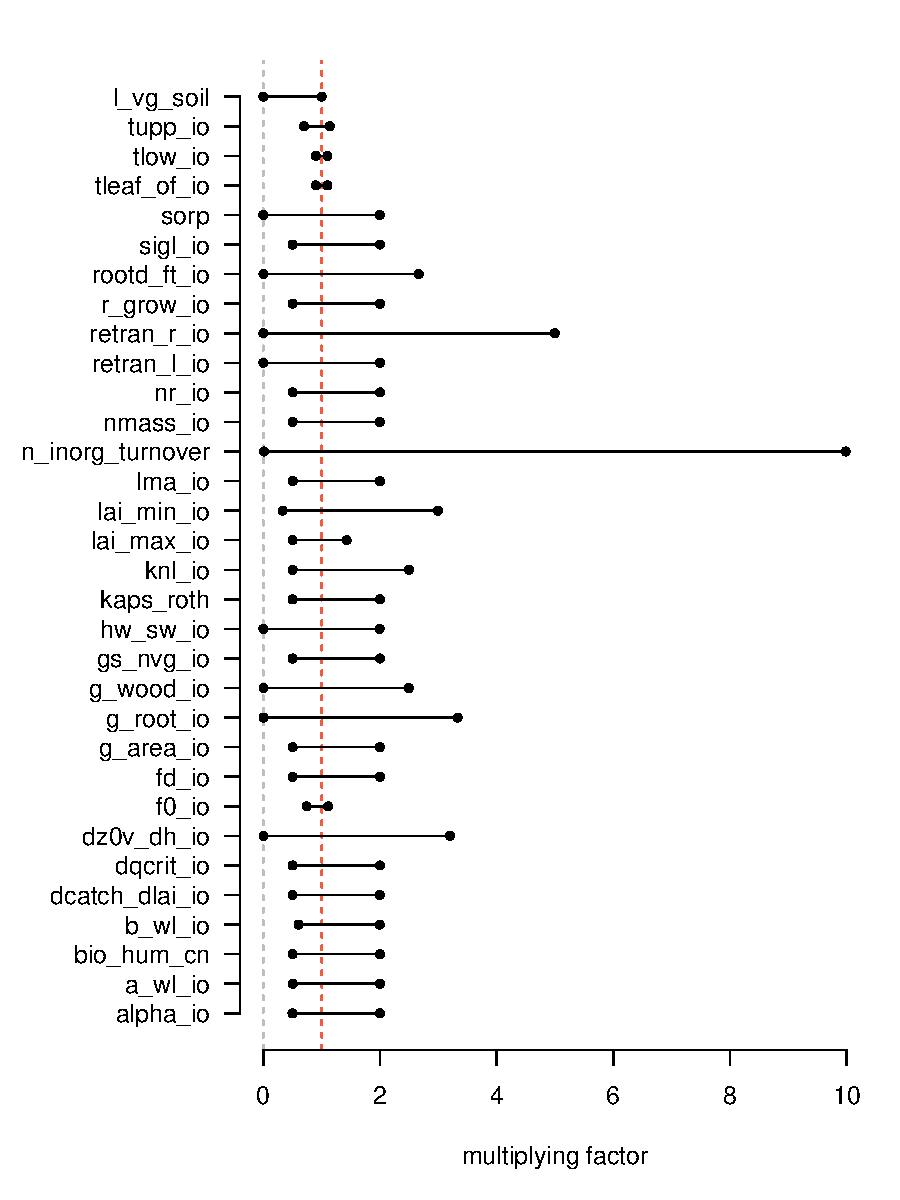
\includegraphics[width=12cm]{./figs/fig01.pdf}
\caption{Parameter multiplication factor ranges the initial ensemble (wave00) design.}
\label{fig:lhs_range}
\end{figure*}

\section{Sequential constraint}\label{sec:sequential_constraint}

Our "iterated refocussing" experiment uses a combination of formal and informal methods to sequentially constrain input parameter space and model behaviour, dependent on both expertise and expectation of the modellers, and on more formal comparison with observational data. An important aim for the initial ensemble is primarily to train a good surrogate model, and therefore we require relatively smooth output across the inputs space, without discontinuities or highly nonlinear behaviour that might bias an emulator. Our initial constraint procedures set out to achieve this.

Our initial (wave00) ensemble of 499 members is sequentially constrained; to "Level0" by removing 24 ensemble members which do not run (see sect. \ref{ssec:failure-analysis}), to "Level 1" by removing the 50 remaining ensemble member outside of the threshold in $F0$ identified in sect. \ref{ssec:failure-analysis}, and "Level 1a" by removing the 64 remaining members outside the threshold in $b\_wl\_io$. This leaves us with a wave00 "level 1a" ensemble of 361 members that at least run and have a minimally functioning carbon cycle.

\subsection{Failure analysis}\label{ssec:failure-analysis}

We analyse the ensemble to remove ensemble members and corresponding parts of parameter space that very obviously cannot hope to produce a useful simulation of the carbon cycle. First, we map ensemble members where the simulator failed to complete a simulation, perhaps due to numerical error (termed "failed"). Second, we identify parts of parameter space where important parts of the carbon cycle are completely missing - that is, basic carbon cycle quantities are at or close to zero at the end of the run (termed "zero carbon cycle"). For this second class, we choose a threshold of mean modern global NPP close to zero ($<10^{-5}$).
The nature of perturbed parameter ensembles is that there is often a setting of some parameters that makes up for a poor choice of a particular parameter, and so outright and easily identifiable thresholds for failure in the marginal range of a particular parameter are rare. However, careful visualisation and analysis can give the modeller a good idea of regions of parameter space that can be removed, or parameters that the model is particularly sensitive to.

In fig. \ref{fig:run-failure-pairs}, we see a pairs plot of "failed" runs (upper right panels) and, "zero carbon cycle" panels (lower left panels). The plot shows the two-dimensional projections of run failures against each pair of inputs, allowing visual identification of inputs that control failures, and any potential two-way interactions.

For example, we can see that both $f0\_io$ and $b\_wl\_io$ have important thresholds, beyond which there is almost no chance of a functioning carbon cycle. As there appears little to no interaction between these two, this presents as a nearly-blank plot at the intersection of the parameters on the plot (row 8, column 4), with inputs identifying zero-carbon runs around the edges of the sub plot. High values of $b\_wl\_io$ results in unphysical allometric scaling of vegetation height to biomass (e.g. 250m tall trees!).

%*[$f0\_io$ is the ratio of internal to external co2 partial pressure - presumably low values lead to no NPP but it appears to be the other way round in the diagram - to check ]*
% Answer: threshold behaviour, there doesn't seem to be a strong relationship between f0 and NPP.
% https://dougmcneall.github.io/jules_ppe/constrain-JULES-ES-1p0.html


\begin{figure*}[t]
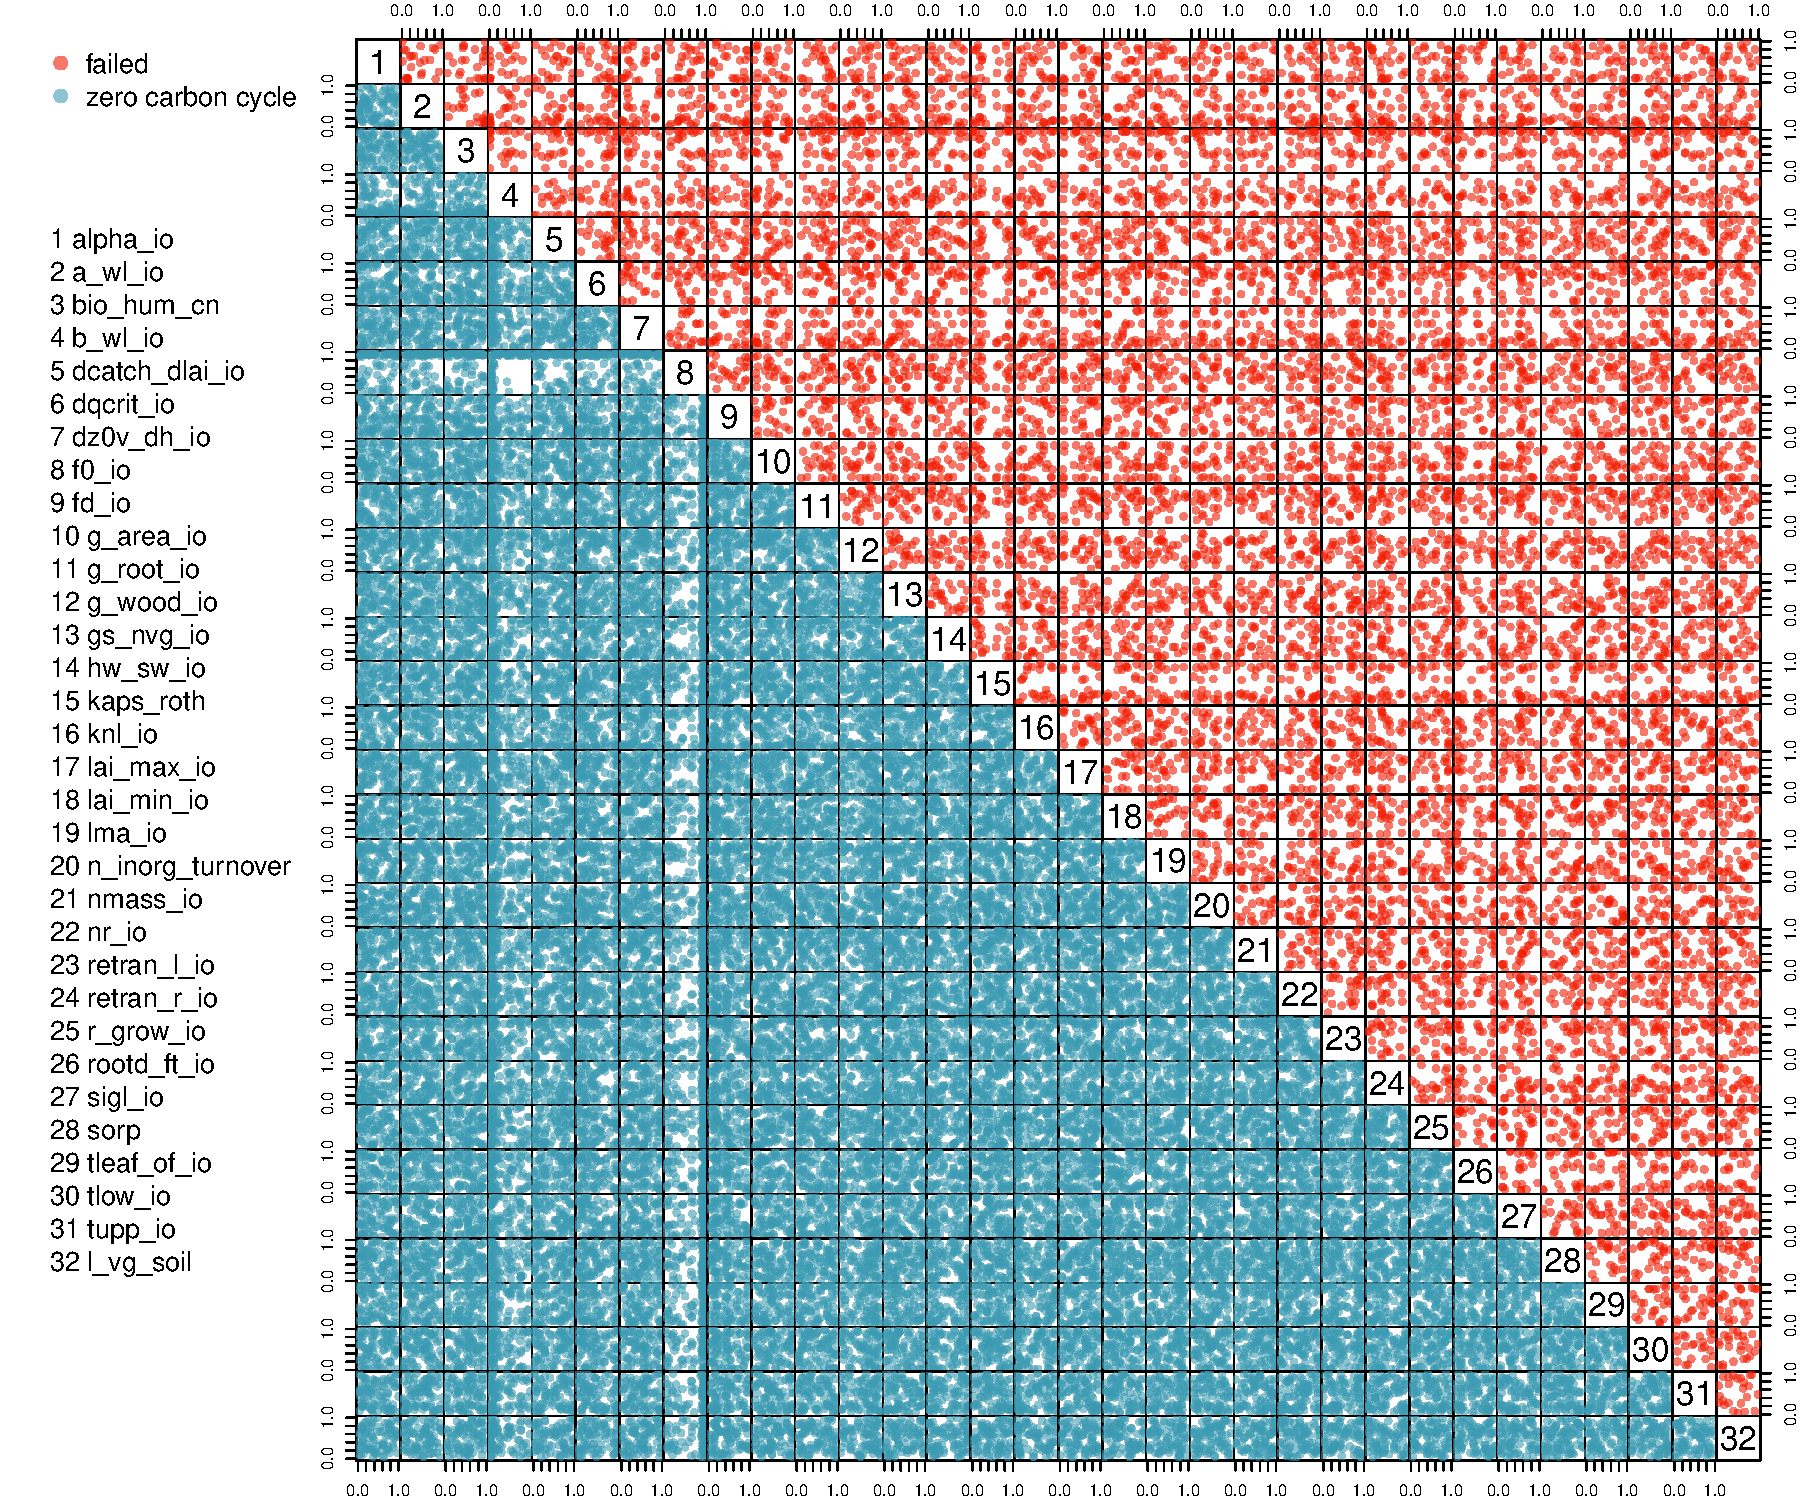
\includegraphics[width=12cm]{./figs/fig02.pdf}
\caption{Two-dimensional projections of the input parameter values in normalised input space of the ensemble members that failed or had zero carbon cycle.}
\label{fig:run-failure-pairs}
\end{figure*}


\subsection{First wave results (level1a constraint)}\label{sssec:level1a}

The globally averaged carbon cycle and land surface behaviour of the level1a - constrained ensemble can be seen in fig. \ref{fig:carbon-cycle-timeseries-waves-constrained}, and anomalies compared to the average of the first 20 years of the runs can be seen in fig. \ref{fig:carbon-cycle-timeseries-anomaly-waves-constrained}, in the blue lines.

\begin{figure*}[t]
\includegraphics[width=12cm]{./figs/fig03.pdf}
\caption{Timeseries of absolute carbon cycle quantities in the JULES ensemble at increasingly strict levels of constraint.}
\label{fig:carbon-cycle-timeseries-waves-constrained}
\end{figure*}

%%% TWO-COLUMN FIGURES
%
%%f
\begin{figure*}[t]
\includegraphics[width=12cm]{./figs/fig04.pdf}
\caption{Timeseries of carbon cycle anomaly quantities in the JULES ensemble at increasingly strict levels of constraint.}
\label{fig:carbon-cycle-timeseries-anomaly-waves-constrained}
\end{figure*}

The ensemble displays a very wide range of both absolute levels and changes in a selection of carbon cycle and land surface properties, compared to the model run at standard settings (black). For example, global total NPP runs from approximately zero to over 150 GtC/year. Soil carbon stocks are between zero and more than 4000 GtC, and Vegetation stocks range from 0 to over 2000 GtC.

A large number of first wave (wave00) ensemble members have a hugely diminished carbon cycle and carbon cycle stocks compared to the standard member. This can be seen from examining fig. \ref{fig:carbon-cycle-timeseries-waves-constrained} compared to the values of the standard member (black lines). In particular, most ensemble members have a very low tree fraction, and a higher bare soil fraction than the standard member - It seems particularly easy to kill global forests when perturbing parameters. Vegetation and soil carbon levels are also very low in many members. 

Often, perturbing parameters affects the overall level of the carbon cycle property, with its behaviour through time being only a secondary source of variance at the end of the model run. That is, the carbon cycle level at the end of the run is more closely related to its level at the beginning of the run than it is to its change over time. However, there is variability in the behaviour of the carbon cycle over time, as can be seen in fig. \ref{fig:carbon-cycle-timeseries-anomaly-waves-constrained}. Here, we examine a selection of the most important carbon cycle properties, and examine their change in behaviour over time, or anomaly from the starting value. We see for example, that changing the parameters can make soil and vegetation carbon increase or decrease over the simulated century and a half of the model run. 

\subsection{Second wave ensemble}\label{ssec:second_wave}

We can constrain both the historical behaviour of the model and the model parameter input space by comparison of the model behaviour with the expectations of the model developers; with those expectations set by knowledge of observations and, when those are uncertain or unavalable, by first principles and model simulations from independent groups. A simple way to constrain the historical behaviour of the carbon cycle is by removing from the ensemble those model runs (and their corresponding input parameter settings) that lead to seemingly implausible values of basic carbon cycle quantities in the modern era.

We choose a small number of broad constraints that the model must adhere to in order to be considered a valid and useful simulation. The constraints are four basic carbon cycle properties, globally averaged over the final 20 years of the simulations, near the beginning of the 21st century (1995 - 2014). They are net biome production (NBP), net primary production (NPP), and the land surface stocks of soil and vegetation carbon (cSoil and cVeg respectively). We choose generous limits on what might be called valid, roughly in line with the range of the CMIP5 Earth system model multi-model ensemble of opportunity. These constraints are outlined in table \ref{table:level_2_constraints}. We designate these limits the "level 2" constraints.

Only a very small proportion of ensemble members (38 out of 499) conform to the basic "level 2" constraints expected of a useful model by our modeller. We would like to have a larger number of ensemble members in this range, so that any emulator we build has enough detail to be useful, and we can accurately map out viable input space. We wish to run more ensemble members within a valid input space, and so we formally history match to the level 2 space, in order to generate an input design for a second wave of ensemble members. We describe this process in sect. \ref{ssec:history_matching}.

\begin{table*}[t]
\caption{Increasing levels of constraint applied to simulator output during the experiment.}
\label{table:levels_of_constraint}
\begin{tabular}{l r}
\tophline
Level & Constraint  \\ 
\middlehline
Level 0  & simulation completes \\
Level 1 & $F0 < 0.9$ \\
Level 1a & $B\_WL\_IO > 0.15 $ \\ 
Level 2  & NPP, NBP, cVeg and cSoil \\

\bottomhline
\end{tabular}
\belowtable{} % Table Footnotes

\end{table*}


\begin{table*}[t]
\caption{Output limits to be met over the last two decades of simulation to match "Level 2" constraints.}
\label{table:level_2_constraints}
\begin{tabular}{l r r}
\tophline
Constraint & Minimum & Maximum \\ 
\middlehline
NBP & 0 GtC/yr &  10 GtC/yr\\
NPP & 35 GtC/yr & 80 GtC/yr \\
Soil Carbon stock & 750 GtC &  3000 GtC\\ 
Vegetation Carbon stock & 300 GtC & 800 GtC \\

\bottomhline
\end{tabular}
\belowtable{} % Table Footnotes

\end{table*}


\subsection{History matching}\label{ssec:history_matching}

History matching is a process whereby we formally compare the output of the model to observations of the real system, and reject parts of input parameter space where the model is not expected to plausibly simulate reality. Crucially, history matching recognises uncertainty both in the observations of the system, and the model being used to simulate it. We use history matching to constrain the input space of the model, in order to both learn about inputs, and to find an input space which could credibly be used for future projections.

History matching has been used to great effect for constraining complex and computationally expensive simulators in a number of fields, including oil reservoir modelling \citep{craig1996strategies, craig1997pressure}, galaxy formation \citep{vernon2010galaxy, vernon2014observable}, infectious diseases \citep{andrianakis2015bayesian}, and climate modelling \citep{williamson2013history, williamson2015identifying, mcneall2020correcting}.

History matching measures the statistical distance between an observation of a real-world process, and the predicted output of the climate model at an input parameter setting. An input where the model output is deemed too far from the corresponding observation is considered ``implausible'', and is ruled out. Remaining inputs are conditionally accepted as ``Not Ruled Out Yet'' (NROY), recognising that further information about the model or observations might yet rule them as implausible.

A vector representing the outputs of interest of the true land surface properties is denoted $y$. Observations of the system are denoted $z$, and we assume that they are made with uncorrelated and independent errors $\epsilon$ such that 

\begin{equation}
z = y+\epsilon
\end{equation}

The climate simulator is represented as an unknown deterministic function $g(.)$ that runs at a vector of inputs $x$. We assume a ``best'' set of inputs $x^*$ which minimises the model discrepancy, $\delta$, which represents the structural difference between the model and reality. In practice this minimises the difference between climate model output $g(x)$ and observations $z$. We can therefore relate observations to inputs with 

\begin{equation}
z = g(x^*) + \delta + \epsilon. 
\end{equation}

The statistical distance between the simulator, run at a particular set of inputs $x$, and reality is measured using implausibility $I$:

\begin{equation}\label{eq:implausibility}
I^{2} = {\lvert  z - E[g(x)]\rvert}^{2} /  (Var[g(x)] + Var[\delta] +  Var[\epsilon]).
\end{equation}

This equation recognises that there is uncertainty in the output of the simulator, and that this is estimated by an emulator. In this study, we use a Gaussian process emulator, described in appendix \ref{app:emulator}. Distance between the best estimate of the emulator and the observations must be normalised by uncertainty in the emulator $Var[g(x)]$, in the observational error $Var[\epsilon$], and in the estimate of model discrepancy $Var[\delta]$. 

We reject any input as implausible where $I >3$ after Pukelsheim's three-sigma rule; that is, for any unimodal distribution, 95 \% of the probability mass will be contained within 3 standard deviations of the mean \citep{pukelsheim1994three}.

\subsection{Second wave design}\label{ssec:second_wave_design}

We wish to generate design points for the second wave (wave01) which we believe will generate output that is not implausible: that is where $I<3$ according to equation \ref{eq:implausibility}. As seen in the first wave (wave00), randomly sampling from across \emph{a priori} plausible input space generates a large number of ensemble members which do not look like reality. Our strategy to increase the proportion which generate realistic output is to use the Gaussian process emulator to predict model output, generate a large number of potential candidates for new design points, and history match to reject candidates we believe will lead to implausible output.

After building a Gaussian process emulator for each of the four "modern value constraint outputs" (NBP, NPP, cSoil and cVeg), we generate a large number (50,000) samples uniformly from the \emph{a priori} not implausible input space. We calculate $I$ for each of these samples, for each of the 4 outputs. 

To calculate $I$, we set our "observation" as the mid point of the tolerated range set by modeller Wiltshire (see table \ref{table:level_2_constraints}), and assume that the limits correspond to the 95\% range of an implied distribution (i.e. the range of the limits is assumed to cover 4 standard deviations of uncertainty in the assumed distribution). We assume that the expected model discrepancy is zero, and that the uncertainty on model discrepancy is also vanishingly small. In effect, this means that most of the uncertainty budget comes from the emulator and the observations.


From the subset of samples where $I < 3$ (i.e. NROY) for all four outputs, we sample 500 potential design candidates and calculate the minimum distance between them in input space. We do this 500 times, and choose the set with the largest minimum distance. This is to ensure that no two points are too close together, which can cause numerical errors when re-building the Gaussian process emulators. This set is then used to run the second wave ensemble (wave01).

\subsection{Second wave results}\label{ssec:second_wave_results}

A summary of the output of the second wave in the modern constraint variables can be seen in figure \ref{fig:level_2_constraints_hists}, compared to the same output from the first wave, constrained to level 1a. If the history matching process was perfect, 95\% of ensemble members would have output within the specified constraints (denoted by the grey region in the histograms). As there is uncertainty in the emulator, the majority of the second wave ensemble members fall outside of these constraints. Of the 500 new members, we keep back 100 for validation purposes in future studies. of the remaining 400, 128 (32\%) conform to all four constraints, compared with 27 out of 499 (7.4\%) of the initial ensemble.

It is worth noting, however, that the proportion of ensemble members in the second wave that match the constraints is much higher, and that majority of ensemble members in the second wave fall within any one individual constraint. It is only when these constraints are combined that the majority are ruled out. A possible cause of the relatively small number of ensemble members that fall into the level 2 constraints is one or more poor emulators. We investigate this possibility in appendix sect. \ref{app:level_2_pred}, and conclude that this is likely the emulator for cVeg consistently predicting low, particularly for the higher (and more realistic) values of cVeg. The average value of NBP, NPP, cSoil and cVeg has moved up in the second wave. There are no ensemble members that fail to run in the second wave, nor are there any that have a "zero carbon" world, but there are 10 that have numerical problems and unusual values in their timeseries, and these are excluded from our analysis.

\begin{figure*}[t]
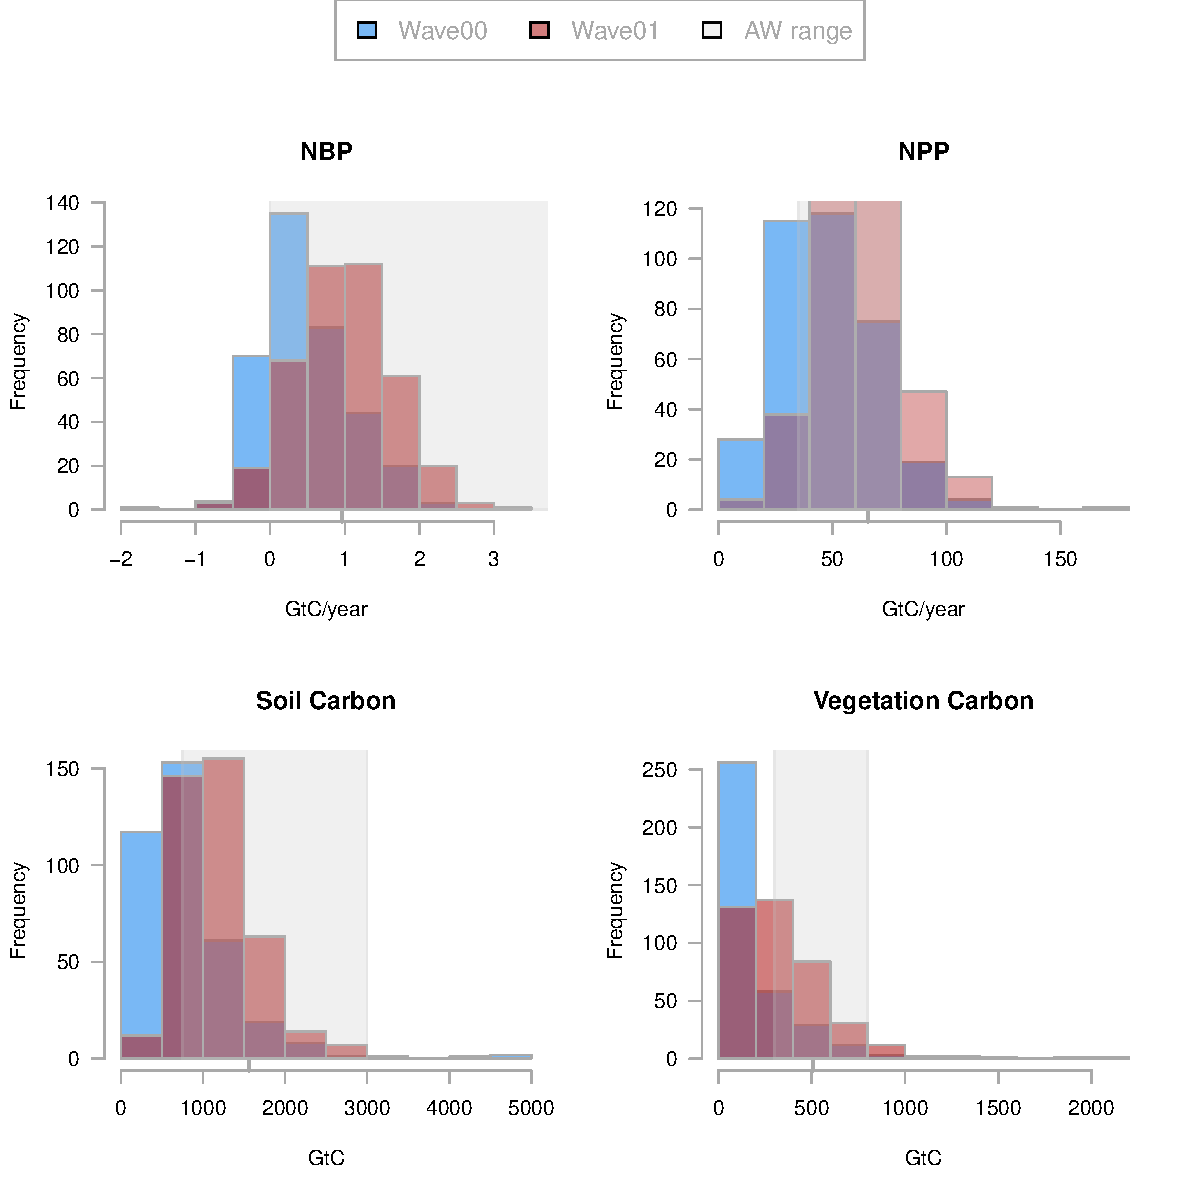
\includegraphics[width=12cm]{./figs/fig05.pdf}
\caption{Histograms of ensemble output for the "constraint outputs", global mean NBP, NPP, cVeg and cSoil, in wave00 (blue) and wave01 (red). Shaded grey region indicates the constraints.}
\label{fig:level_2_constraints_hists}
\end{figure*}
 
\subsection{Induced constraints}\label{ssec:induced_constraints}

We see time series of the second wave ensemble in fig. \ref{fig:carbon-cycle-timeseries-waves-constrained} and anomaly timeseries in fig. \ref{fig:carbon-cycle-timeseries-anomaly-waves-constrained}. The raw wave01 ensemble is coloured red, and the subset of ensemble members that conform to the level 2 constraints is coloured yellow. We can see a considerable constraint (as expected) in the timeseries of the constraint variables. However, we also see a constraints of varying magnitude in leaf area index (LAI), soil respiration (RH), crop harvest carbon flux (fHarvest) tree fraction (treefrac), bare soil fraction (baresoilfrac) and others. Our working hypothesis is that our cVeg constraint enforces a minimum level of tree cover and therefore excludes high cover of other PFTs and bare soil. Such a constraint also seems to exclude low values of LAI. Our NPP constraint likely excludes low harvest flux and low values of soil respiration (RH).

Present day constraints act to constrain historical trends in some of the variables, suggesting that uncertainty in some future projections might also be reduced. We see, for example that constraining present day levels of the carbon cycle variables induces a constraint in NPP trends but not NBP trends. The trend in cSoil is constrained slightly and the biggest historical losses of vegetation carbon are ruled out. Many (but not all) of the ensemble members that lose shrub fraction during the run are ruled out. Ensemble members with high C4 grasses loss are ruled out. However, changes in vegetation carbon or leaf area index are hardly constrained at all.

% at this point, we could look at pairs plots of the ensemble input space that passes the constraints directly. (could use the same colours)




\subsection{Constraining input space with an emulator}\label{ssec:constraining_input_space_emulator}

Constraining the ensemble by directly rejecting implausible members gives us a useful but rough outline of the input space where the model might be said to behave "well". With only 38 ensemble members in the first wave, we were able to outline the valid 32 dimensional input space only very approximately.

\begin{figure*}[t]
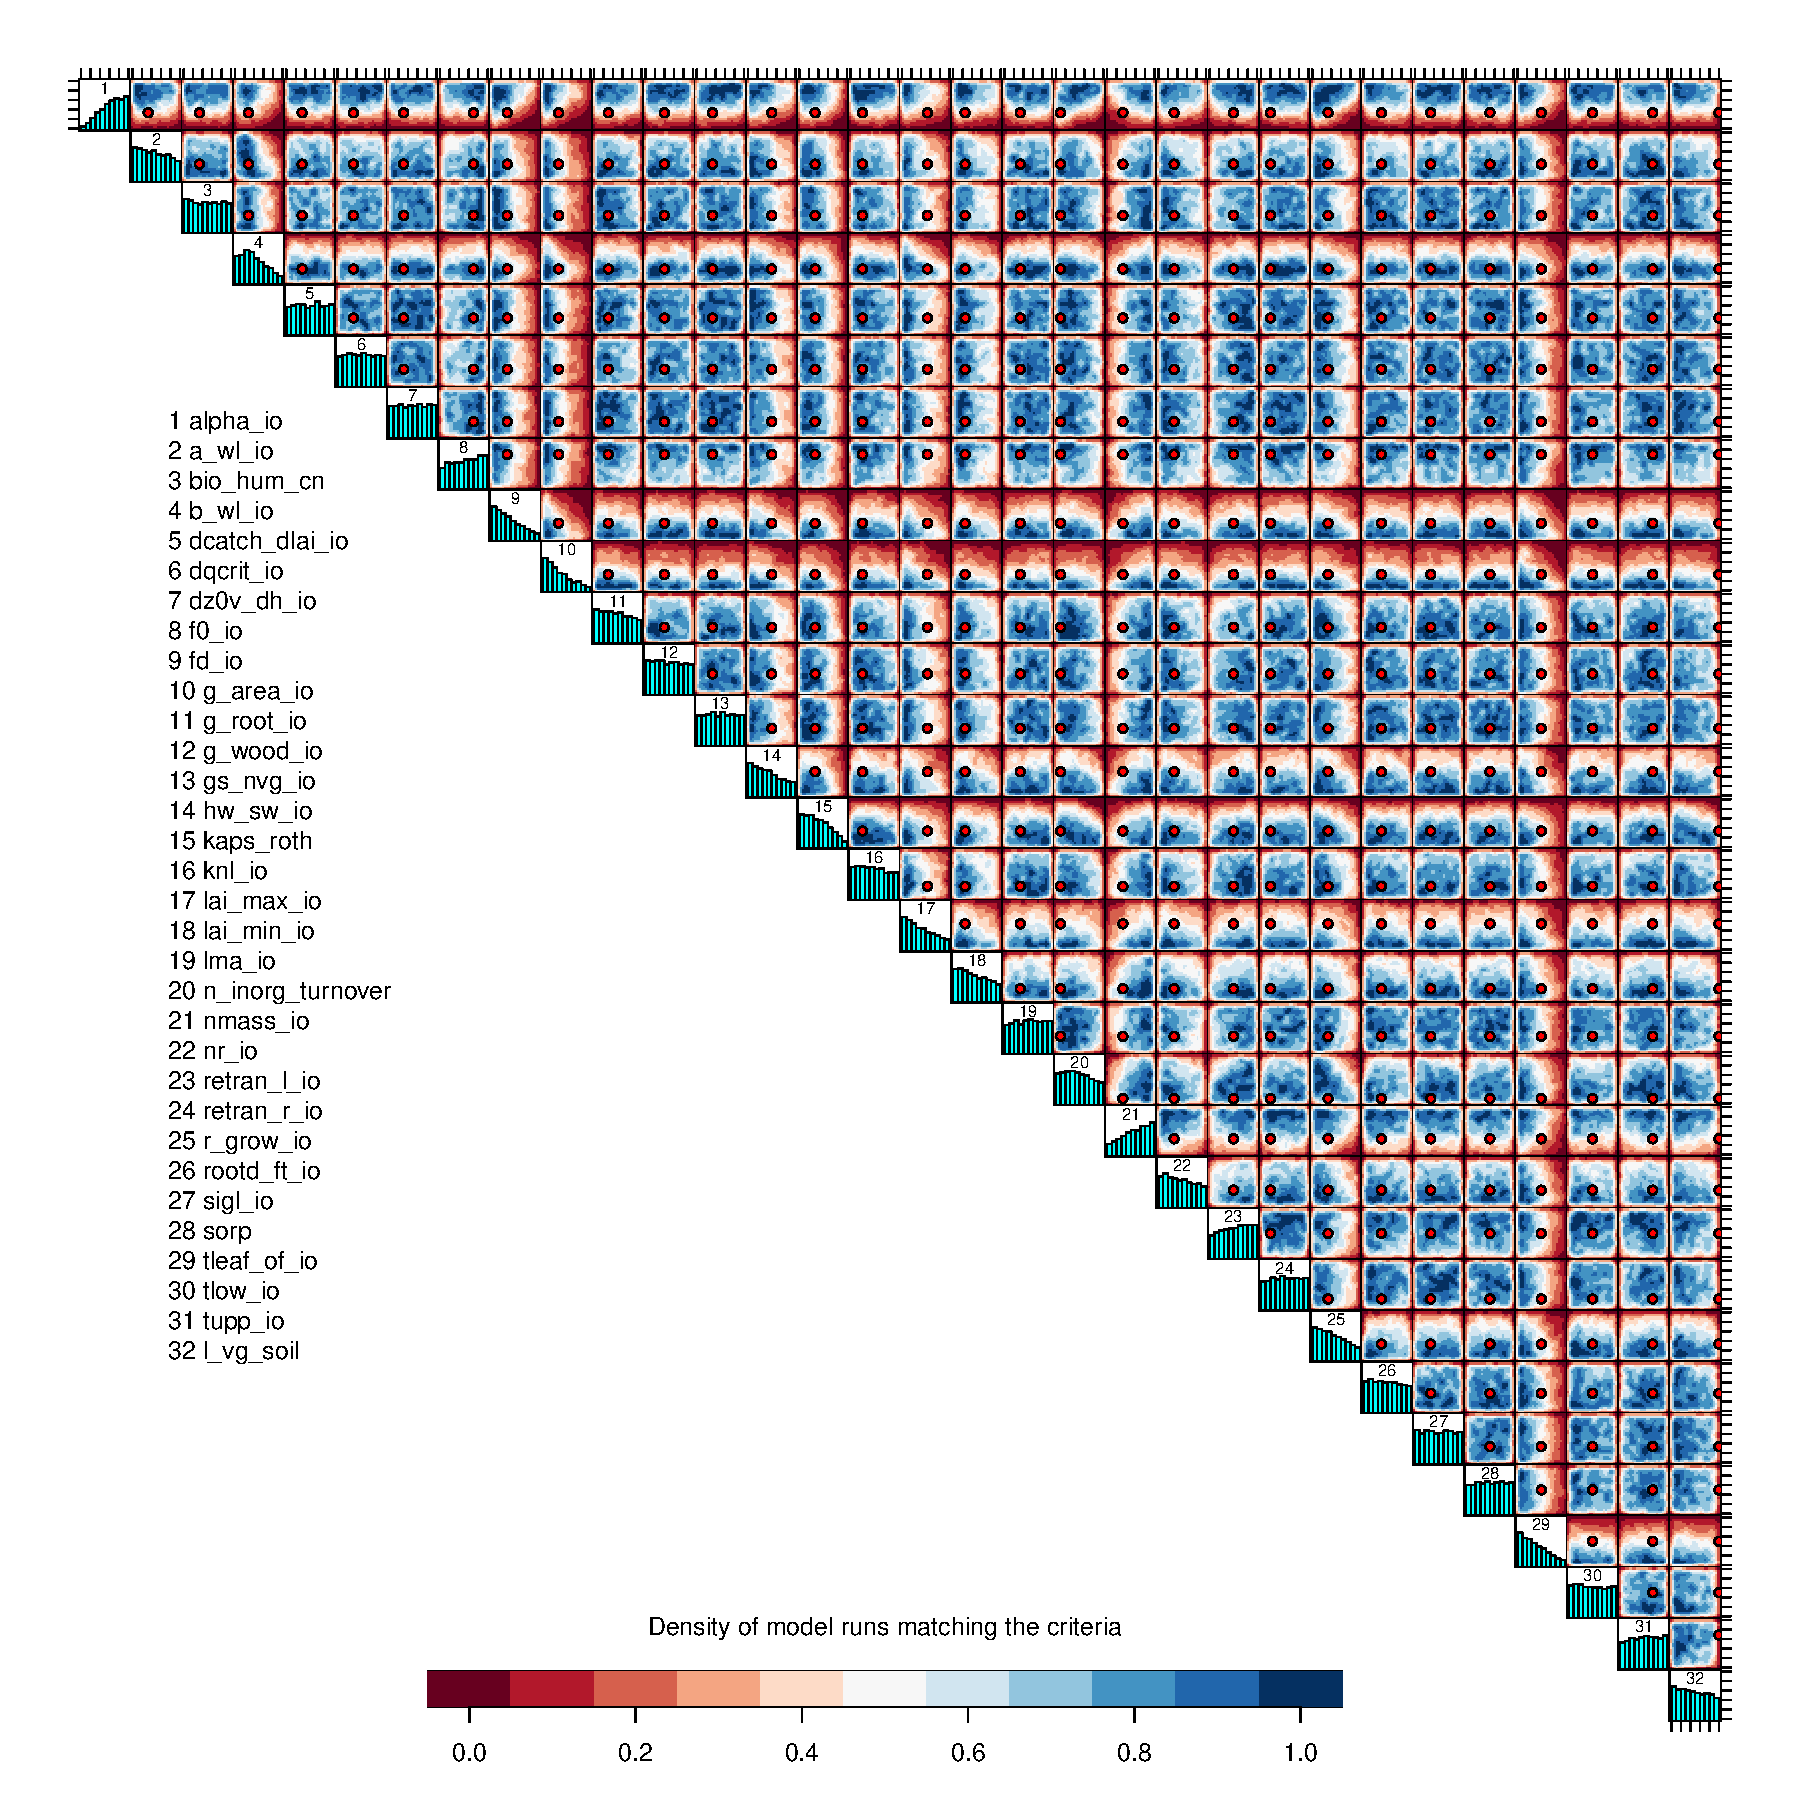
\includegraphics[width=12cm]{./figs/fig06.pdf}
\caption{Two-dimensional projections of the density of input parameter candidates that conform to level 2 constraints. Blue regions have a higher density of points and red regions lower. Marginal histograms indicate the marginal density. Red points mark the standard input parameter value.}
\label{fig:pairs_level2_ix_em_unif_wave00_wave01}
\end{figure*}

We visualise the constrained input parameter space with the help of an emulator. We can use the trained emulator in place of the full simulator JULES-ES-1.0, examining the inputs where the emulator predicts that the simulated outputs would match our constraints. Because the emulator is orders of magnitude cheaper to evaluate, we can take many thousands of samples from input space and predict whether the simulator would match the constraints. This means that diagrams that summarise the input spaces can show densities of input points with a much higher resolution. The trade-off is that the emulator does not perfectly predict simulator output, and so visualisations of constrained input space are approximate. However, we judge that the emulator is accurate enough to provide useful insights, given the error and validation studies in appendix \ref{app:emulator_accuracy}.

We fit a Gaussian process emulator to each of the modern constraint outputs using the 751 members of both ensemble waves that have a non-zero carbon cycle. We take $10^{5}$ samples uniformly from across the original normalised input space, and reject all emulated members where the corresponding mean predicted output does not conform to the level 2 constraints. We plot two dimensional projections of the the density of accepted points in figure \ref{fig:pairs_level2_ix_em_unif_wave00_wave01}, colour coded by relative density. Blue areas show regions where there is a high concentration of accepted points, and we would expect a high probability of a model run in at this input location producing a valid carbon cycle.

We calculate the proportion of space that conforms to the level 2 constraints as approximately the proportion of samples - the large number of samples assures that the sampling uncertainty is small. Approximately 12\% of the initial input space conforms to all four level 2 constraints.

\section{Sensitivity Analysis}\label{sec:sensitivity_analysis}

Global sensitivity analysis calculates the impact of changes in input parameters on simulator outputs, when inputs are perturbed across the entire valid input space. This is in contrast to a local sensitivity analysis, which calculates the impacts of small deviations from a set of default values. The two types of analysis are useful in different contexts: in our case, we have large uncertainties relating to a number of inputs, model processes and observations, and so a global sensitivity analysis as a form of "screening" of important input parameters is appropriate.

We use a set of Gaussian process emulators, fit to each of the JULES-ES-1.0 land surface summary outputs to perform two types of global sensitivity analysis. We use the set of Gaussian process emulators fit to each of the outputs used for our "level 2" constraint for a third kind of sensitivity analysis. Each type of sensitivity analysis tells us different things about the relationship between the inputs and outputs of JULES-ES-1.0. At the end of this section, we summarise the results of all three types of sensitivity analysis in order to suggest which inputs might be prioritised in any future experiment.

Our aim is to give the modeller quantitative information on which inputs affect which outputs, to direct effort for reducing model biases and errors, and to indicate regions of parameter space where the model might perform better. We might identify parameters which have a direct impact on model output which does not conform to observations, identify groups of parameters withing a poorly performing process, or help modellers sample uncertainty in other model applications..

\subsection{Global one-at-a-time Sensitivity}\label{ssec:sa_oaat}

A one-at-a-time (OAAT) sensitivity gives a simple and easy-to-interpret measure of the impact of each input on a variety of outputs, but does not include the effects of any interactions between inputs (for example, a non-linear change in model outputs as two or more inputs vary together).  

An OAAT analysis can be completed with a relatively small number of model runs - for example, a low, middle and high run for each parameter in our 32 input dimension example would take fewer than 100 runs. However, using an emulator allows us to better characterise the response of the model across the entire range of each parameter, which would take many more dedicated runs if completed using just the model.

We fit a Gaussian process emulator to each global summary output, both as a ``modern value'' (mean of 1995 - 2014), and as an ``anomaly" (change since 1850-1869). We use the 751 members from both wave00 and wave01 that conform to the level1a constraints, being as wide an input space as possible without significant model failure.

We sample from the input space in a one-at-a-time fashion: each input is sampled uniformly across it's input space, with all other inputs held at standard values (note, these are often not the central value when normalized to 0-1 range). The variance of the mean emulated output as each input is varied is then used as a measure of the sensitivity of that output to the corresponding input. Variance is used as opposed to magnitude of change, as we expect some model outputs not to rise or fall monotonically as an input varies.

Different model outputs are clearly sensitive to different model inputs, and so we also seek ways of summarising sensitivity across model outputs. One method is simply to find the mean effect across model outputs. Sensitivities are normalised so that they lie in a $[0 -1]$ range for each output. Summary measures for each input are then averaged across all outputs, and the plotted inputs are ranked by their average influence across all outputs. Individual sensitivities and summaries can be seen in fig. \ref{fig:oat_var_sensmat_level1a_wave01_Y} for the modern value, and in fig. \ref{fig:oat_var_sensmat_level1a_wave01_Anom} for the change over the historic period of the ensemble. We see that for both modern value and anomaly, by this measure only half or fewer of the inputs have discernible impact on global outputs.

\begin{figure}[t]
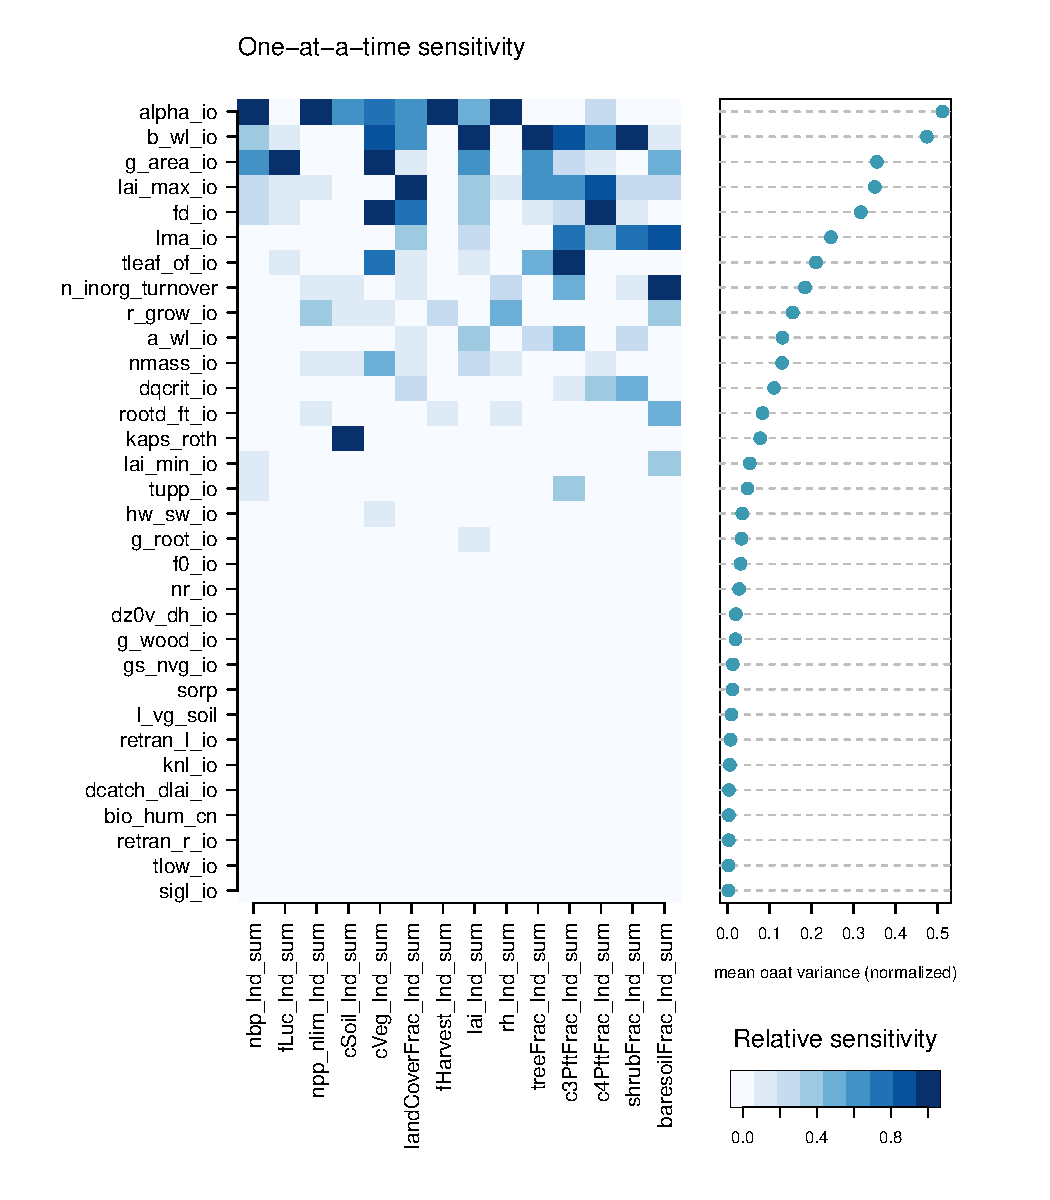
\includegraphics[width=12cm]{./figs/fig07.pdf}
\caption{One-at-a-time sensitivity summary for global summary ``modern value" output.}
\label{fig:oat_var_sensmat_level1a_wave01_Y}
\end{figure}

\begin{figure}[t]
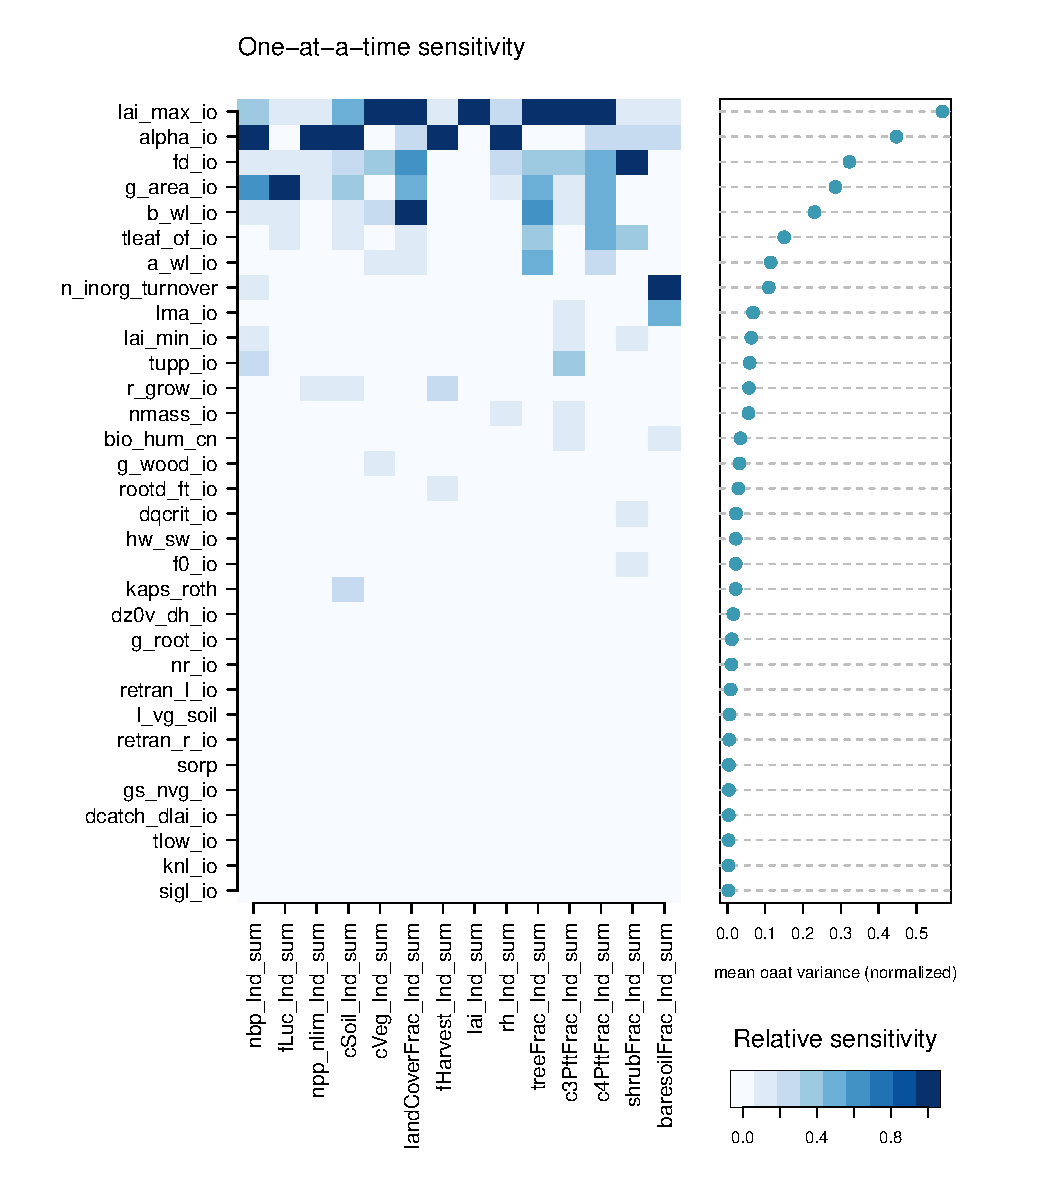
\includegraphics[width=12cm]{./figs/fig08.pdf}
\caption{One-at-a-time sensitivity summary for global summary ``anomaly" (change since 1850-1870) output.}
\label{fig:oat_var_sensmat_level1a_wave01_Anom}
\end{figure}

\subsection{Sensitivity of constraint outputs}\label{ssec:sa_constraint_outputs}

We add detail to our one-at-at-time sensitivity of important outputs - those that we use for constraining JULES-ES-1.0 in figure \ref{fig:Y_oaat_const_level1a_wave01_scaled_norm}. We plot the emulated mean of the each of four outputs - NBP, NPP, vegetation carbon and soil carbon, as each parameter in increased from its minimum to maximum range. Uncertainty bounds from the emulator predictions are not plotted, in order to more clearly see the estimated main effect of each parameter.

For each input, we can see the default value as a vertical dashed line. This plot indicates how deficiencies in the model output might be corrected by altering individual parameters. For example, the fact that many ensemble members have low vegetation carbon might be countered by increasing $alpha\_io$ or $nmass\_io$, or reducing $g\_area\_io$ or $tleaf\_io$. Of course, these alterations will not be without impact on other model outputs, changes in which might be countered elsewhere, or must be weighted against improvements in a particular output.

\begin{figure*}[t]
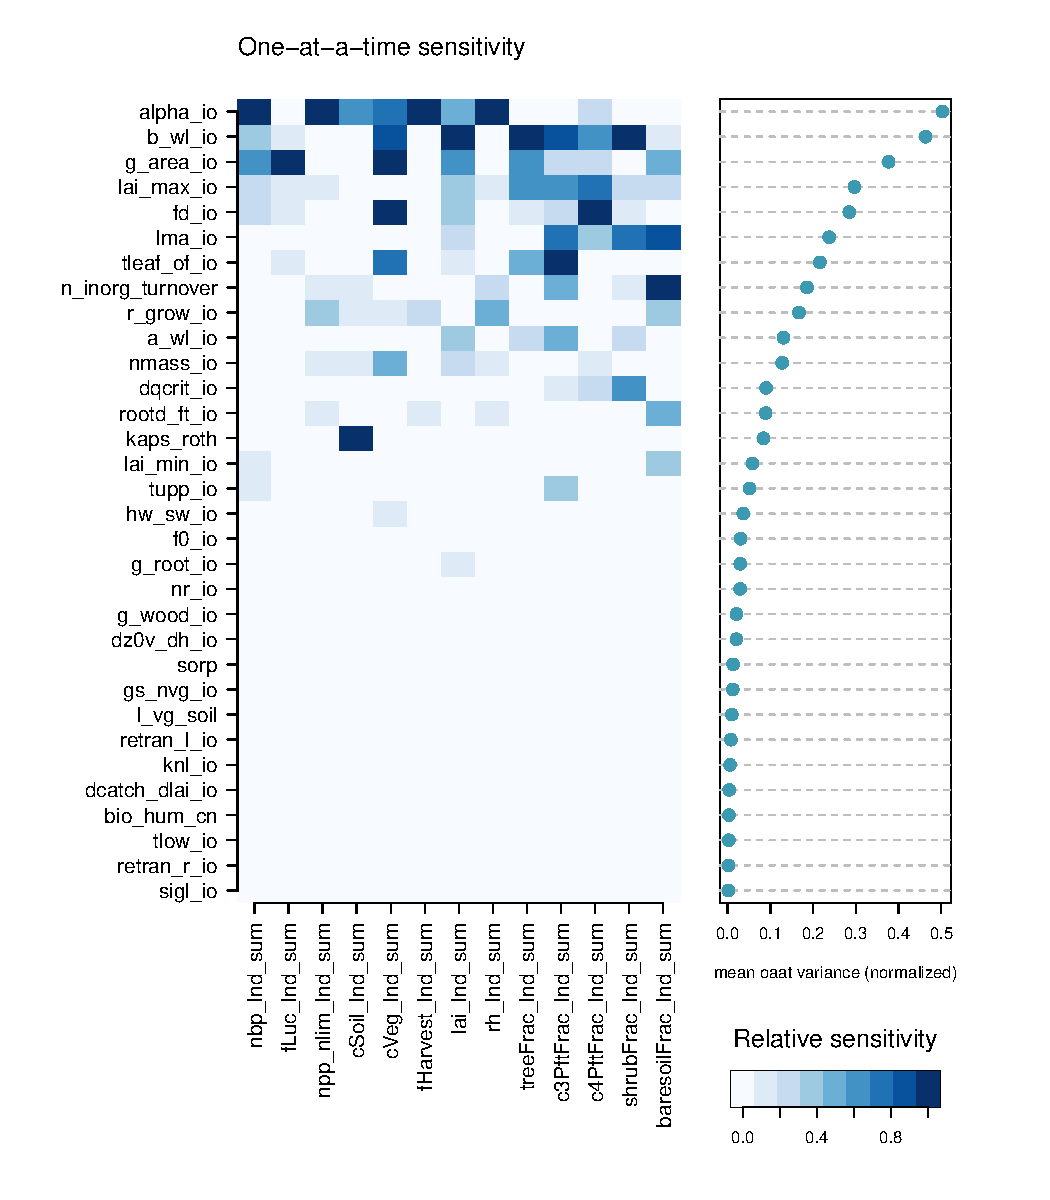
\includegraphics[width=12cm]{./figs/fig09.pdf}
\caption{One-at-a-time sensitivity summary for global summary of the ``modern value" of the constraint variables (nbp, npp, cVeg, cSoil)}
\label{fig:Y_oaat_const_level1a_wave01_scaled_norm}
\end{figure*}

\subsection{FAST sensitivity analysis}\label{ssec:sa_fast}

We use Fourier Amplitiude Sensitivity Test (FAST) as a further measure of global sensitivity of the model outputs to its inputs. The test is administered as the FAST99 algorithm of \cite{saltelli1999sensitivity}, through the R package Sensitivity \citep{Rpackage2015sensitivity}. Again, this algorithm requires a large number of model runs, and so we use emulated model outputs in place of dedicated model runs, as previously used in \cite{mcneall2020correcting, mcneall2016impact, carslaw2013large}. This comes at the cost of a risk of inaccuracy, as the emulated model outputs won't perfectly reproduce the true model runs at the corresponding inputs. However, the emulator is shown to work adequately for the model outputs in appendix \ref{app:emulator_accuracy}. 

A FAST gives both first order and interaction effects: we sum these together to calculate a total sensitivity index, to make showing the results across a large number of outputs simpler. Individual results for FAST can be seen in appendix \ref{app:sa_fast}, and the summarised results are used in our analysis in sect. \ref{ssec:sa_ranking}


\subsection{Monte Carlo Filtering}\label{ssec:sa_MCF}

Monte Carlo filtering (MCF) is a type of sensitivity analysis that integrates well with our aim of constraining model behaviour given a large ensemble using ensemble member rejection, or history matching. The idea of MCF is to identify inputs that have an influence on whether the behaviour of the model falls within or outside acceptable bounds. This is done by splitting samples of model behaviour into those that do or don't meet some constraint, and then summarising the difference between the cumulative distributions of the corresponding input variables. The larger the difference between the cumulative distributions, the more influence the parameter has on whether the model passes the constraint.

A description of MCF and its uses can be found in \cite{pianosi2016sensitivity}. \cite{mcneall2020correcting} uses MCF to estimate parameter sensitivity in the land surface model element of a climate model of intermediate complexity.

We use a Gaussian process emulator to allow a much larger set of samples from the input space, in order to make the MCF process more efficient, at the cost of inaccuracy if the emulator is poor. We train a Gaussian Process emulator on each of the four "constraint outputs", using the 751 ensemble members from both wave00 and wave01 that pass the level1a constraints. We draw a large sample of 10000 parameter combinations, uniformly from the level1a input parameter distributions. We use the emulator to estimate the true model output for each of the four "constraining variables", NPP, NBP, cVeg and cSoil at these parameter values. We perform a two-sample KS test on the cumulative distributions of those input samples where the mean of the emulator predicts that the model would be within or outside of the modellers level 2 constraints. We use this KS statistic as an indicator of the sensitivity of the model output to each input. We summarise the sensitivity in fig. \ref{fig:MCF_sensmat_Yconst_level1a_wave01}.

\begin{figure}[t]
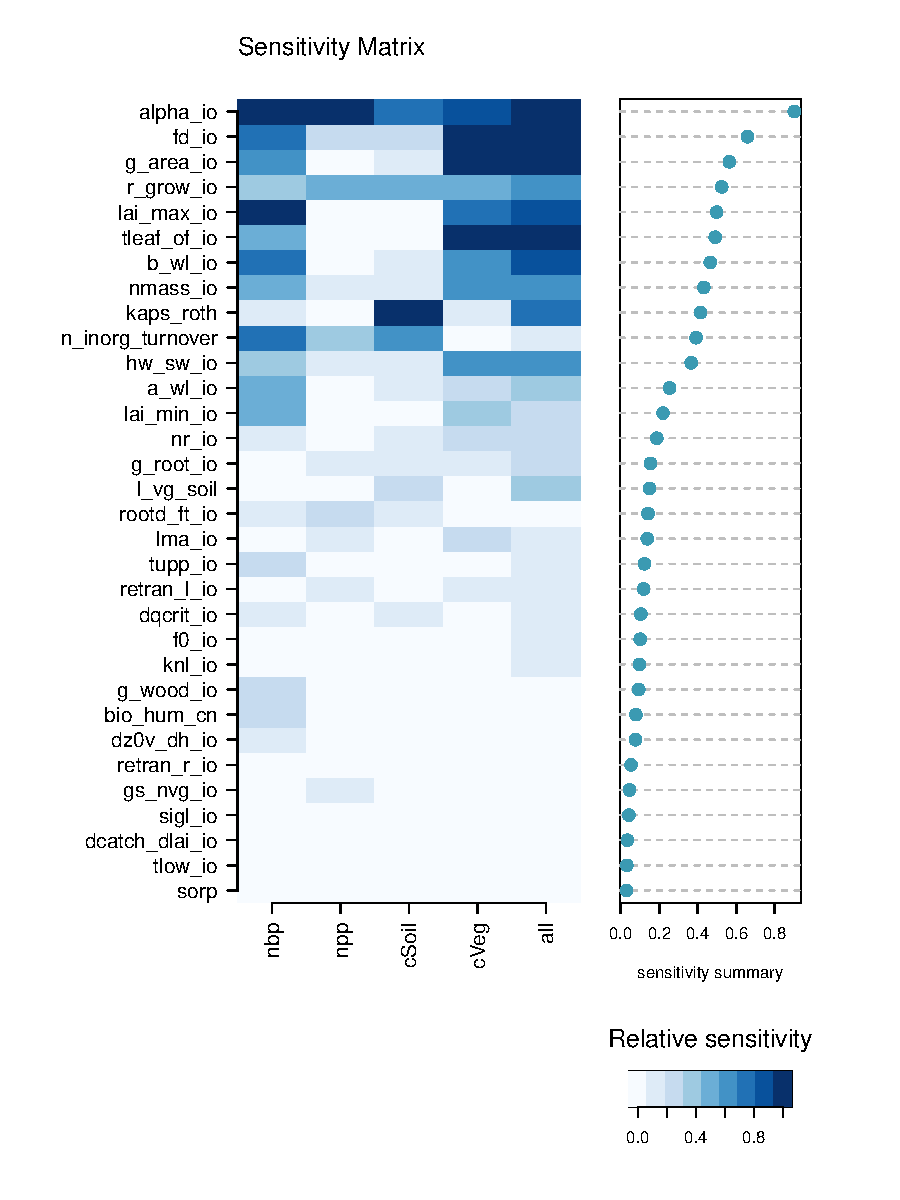
\includegraphics[width=12cm]{./figs/fig10.pdf}
\caption{Monte Carlo filter sensitivity summary for global summary of the ``modern value" of the constraint variables (nbp, npp, cVeg, cSoil)}
\label{fig:MCF_sensmat_Yconst_level1a_wave01}
\end{figure}

\subsection{Screening input variables by  ranking}\label{ssec:sa_ranking}

Which parameters would we include in a subset of parameters for a new ensemble?  One way to choose might be to exclude those parameters which are inactive - those that have a small or no effect on \emph{any} model output of interest, under any of our tested measures of sensitivity. For this ensemble we screen out these ``inactive inputs" by ranking the inputs using each of the sensitivity measures. We can test OAT and FAST SA for both ``modern value'' and ``anomaly'' for the entire set of inputs. We can test Monte Carlo Filtering for the set of ``constraint outputs" that we measure against real-world observations (or modellers expectations).

A conservative strategy excludes only those inputs that are consistently ranked lowest, that is those with the lowest miniumum ranking (or those that have highest value of the rank). While we might choose a number of strategies for weighting of outputs to prioritise input sensitivity, a good start might be to focus on the constraint outputs, later moving towards other output comparisons. We see for example in table \ref{tab:sensitivity_ranks}, that 17 of the parameters never appear in the top 10 most important inputs, for any measure. Depending on our criteria for any new design, we would preferentially disregard inputs that never achieved a high rank.

Using different measures of sensitivity makes our decisions more robust. However, a potential problem with the approach is that all the sensitivity analysis analyses share a Gaussian process emulator, and so will be sensitive to any errors or biases in that shared emulator. It is crucial that model developers are satisfied with the performance of the emulator across the relevant parts of input parameter space, and its associated outputs.

% latex table generated in R 3.6.3 by xtable 1.8-4 package
% Fri May 27 16:02:44 2022
\begin{table}[ht]
\centering
\begin{tabular}{rrrrrrr}
  \hline
 & OAT\_modern\_value & FAST\_modern\_value & OAT\_anomaly & FAST\_anomaly & MCF\_modern\_value & min\_rank \\ 
  \hline
alpha\_io & 1 & 1 & 2 & 1 & 1 & 1 \\ 
  lai\_max\_io & 3 & 5 & 1 & 3 & 7 & 1 \\ 
  b\_wl\_io & 2 & 2 & 5 & 2 & 6 & 2 \\ 
  fd\_io & 5 & 4 & 3 & 5 & 2 & 2 \\ 
  g\_area\_io & 4 & 6 & 4 & 6 & 3 & 3 \\ 
  n\_inorg\_turnover & 7 & 3 & 8 & 4 & 4 & 3 \\ 
  r\_grow\_io & 9 & 8 & 12 & 7 & 5 & 5 \\ 
  lma\_io & 6 & 7 & 9 & 12 & 20 & 6 \\ 
  tleaf\_of\_io & 8 & 11 & 6 & 16 & 8 & 6 \\ 
  a\_wl\_io & 10 & 9 & 7 & 9 & 13 & 7 \\ 
  bio\_hum\_cn & 29 & 26 & 14 & 8 & 18 & 8 \\ 
  hw\_sw\_io & 17 & 15 & 19 & 15 & 9 & 9 \\ 
  kaps\_roth & 14 & 13 & 20 & 14 & 10 & 10 \\ 
  lai\_min\_io & 15 & 14 & 10 & 11 & 12 & 10 \\ 
  nmass\_io & 11 & 10 & 13 & 10 & 11 & 10 \\ 
  tupp\_io & 16 & 18 & 11 & 13 & 16 & 11 \\ 
  dqcrit\_io & 12 & 12 & 18 & 17 & 19 & 12 \\ 
  rootd\_ft\_io & 13 & 16 & 16 & 20 & 15 & 13 \\ 
  nr\_io & 20 & 21 & 23 & 28 & 14 & 14 \\ 
  g\_wood\_io & 22 & 22 & 15 & 19 & 21 & 15 \\ 
  f0\_io & 18 & 17 & 17 & 18 & 26 & 17 \\ 
  l\_vg\_soil & 23 & 25 & 25 & 32 & 17 & 17 \\ 
  g\_root\_io & 19 & 19 & 22 & 22 & 24 & 19 \\ 
  retran\_l\_io & 26 & 20 & 24 & 24 & 22 & 20 \\ 
  dz0v\_dh\_io & 21 & 24 & 21 & 21 & 25 & 21 \\ 
  gs\_nvg\_io & 24 & 23 & 29 & 23 & 27 & 23 \\ 
  knl\_io & 27 & 28 & 31 & 30 & 23 & 23 \\ 
  sorp & 25 & 31 & 27 & 31 & 28 & 25 \\ 
  tlow\_io & 30 & 29 & 30 & 25 & 30 & 25 \\ 
  retran\_r\_io & 28 & 27 & 26 & 27 & 29 & 26 \\ 
  sigl\_io & 31 & 32 & 32 & 26 & 31 & 26 \\ 
  dcatch\_dlai\_io & 32 & 30 & 28 & 29 & 32 & 28 \\ 
   \hline
\end{tabular}
\caption{Summary sensitivity ranks for all carbon cycle outputs, modern value and anomaly, for three different types of sensitivity analysis.}
\label{tab:sensitivity_ranks}
\end{table}


%%% TWO-COLUMN FIGURES

\section{Discussion}\label{sec:discussion}
In this section, we discuss the results of the constraint process and the sensitivity analysis, and what they tell us about the model.

\subsection{Lessons learned}\label{ssec:lessons}

As an exploratory and no-regrets analysis, a key outcome of this experiment is to identify the lessons learned from it, if we would do things differently if we did the experiment again, and what we might take from it to future experiments.

First, would we use  the "top-down" or "data-led" approach - where we perturb all inputs simultaneously, across wide parameter ranges, and constrain with global mean output - again? If we did, could it be improved? This approach provides a rapid and efficient first look at how model parameters influence global output. It's useful for an initial screening parameters, to see which inputs broadly do or do not effect our outputs of interest. It reduces the chances that there may be some unidentified parts of input space where the model would perform better - perhaps we have some discrepancy that can easily be resolved through tuning. The top-down approach might help us set parameter boundaries in situations where there is not strong prior knowledge about what parameters should be.

However, the approach has its limitations and inefficiencies. First, as we see in sect. \ref{sssec:level1a}, a lot of runs fail to complete or have highly unrealistic output (e.g. zero carbon cycle) in the initial ensemble. Only a very small number (less than 10\%) came within the generously wide observational constraints on output.  This was perhaps inevitable, given the approach of halving and doubling the most unknown inputs. Further, the halving and doubling approach leaves the standard member far from the centre of the ensemble, which can perhaps lead to an overemphasis on parts of the input parameter space that were, in hindsight, unlikely to produce good output.

A more careful initial expert elicitation of input parameters might help to target more realistic uncertainty bounds for these parameters, although at a cost of more "human time" spent on the elicitation process, and a higher chance of missing good (but \emph{a priori} unlikely) parts of parameter space. While these kind of experiments can effectively trade computation and analysis time for setup time, the optimal balance of these is often unclear until after the experiment.

With so many free parameters, there are often ways to offset any model discrepancy that can be attributed to a certain parameter, by adjusting another parameter. In this case, it becomes hard to rule out the marginal limits of a parameter when there is always another parameter whose impact can offset it. This means it is difficult to advise modellers on hard constraints for their input parameters. Many constraints will be joint, that is, they will depend on the plausible setting of other parameters. We often see with this kind of setup, a constraint that has ruled out the vast majority of input space as inconsistent with the observations, yet has not ruled out any input space for individual parameters.

How could this problem be addressed? One way of shrinking down marginal space might be to add more data comparisons - increasing the chance that a parameter will be deemed implausible in a history matching exercise, for example. A problem with adding more data until much of input space is ruled out however, is that the chance of an unidentified but significant model discrepancy goes up, particularly if some parts of the climate model are deemed more important, and may have had more development attention than others. In this scenario, a significant model error could lead to analysts unjustifiably ruling out parameter space that should be retained.

A counter to this problem might be found in a sequential approach. Perhaps by targeting particular outputs (and inputs) that are deemed more important in order to get right, before proceeding to data-observation comparisons where relationships are more uncertain. The later data-observation comparisons would carry less weight, and a modelling judgement could be made as to the cut-off point where the analysis continued to add value. Our sensitivity analysis might also help here - narrowing down the most important inputs to perturb in a repeat (or continuation) of the experiment could significantly simplify the input parameter space under investigation.

Another strategy might be a simple "vote" system of constraints, whereby an input is excluded if a number of model outputs fail to meet expectations at a particular input, or a more involved history matching process. A number of multivariate approaches to history matching have been taken in the past, usually either using a maximum value of implausibility, or using a mean squared error approach to calculate an overall implausibility of an input (see eg \cite{vernon2010galaxy}).

\conclusions[Conclusions and further work]\label{sec:conclusions}  %% \conclusions[modified heading if necessary]

In this study we were able to produce a perturbed parameter ensemble of land surface simulations and associated parameter sets using JULES-ES-1.0, consistent with our understanding and observations of the true behaviour of the land surface. 

 An initial design, purposely chosen to produce a wide range of ensemble behaviour, generated only a very small number of members (37/499) that would conform to a set of four basic constraints on global carbon cycle and land surface properties. In this "first wave" of model simulations, there were identifiable marginal limits for parameters $b_wl_io$ and $f0_io$ that caused the simulation to fail, or to produce zero-carbon-cycle climates. These limits were quite near the initial design limits and removing outliers therefore didn't shrink input space much.
 
 We were able to train Gaussian process emulators of global mean summaries of many land surface properties, with mean absolute errors all less than 10\% of the span of the ensemble. After using the emulators to predict outputs that would fall within reasonable constraints in the four key outputs, 128 of 400 members of a second wave of simulations complied with the constraints. Emulator performance improved for most outputs after adding data from the second wave to the training set - particularly for those members that passed the level 2 constraints. This means that analyses will be more accurate and have less uncertainty than they would have when training with only the initial ensemble. Constraining input space to the four basic (Level 2) using the emulator removed 88\% of initial input parameter space, but marginal ranges were hard to constrain. There were "induced constraints" on a number of outputs (but not all), when the ensemble output is constrained using the 4 basic properties.
    
We used 3 types of global sensitivity analysis to identify the most (and least) important parameters.  A number of inputs which have very little impact on global output were identified, and would be recommended to be excluded from further analyses in order to simplify the input space and improve emulator performance. Detailed information on the relationship between individual parameters and global mean outputs will be useful to modellers identifying ways to improve the simulator. A focus on the key uncertain parameters will be useful for modellers, to inform future improvements of JULES, ahead of the next generation Earth system models.

The potential of observations to further constrain input parameter space could and should be explored. Both more waves of simulations - further improving emulators and reducing uncertainty - and new observations of unconstrained outputs could be tried. Care must be taken to ensure that adding more observations doesn't unduly increase the chances of including an unidentified simulator discrepancy.

We might identify parts of parameter space where the model does better at reproducing observations. Regions that produce more realistic carbon vegetation (cVeg) for example, or airborne fraction could be targeted in an optimisation or calibration routine. A simple analysis could illustrate parts of input parameter space that do better than the standard ensemble member.

Finally, we could use sensitivity analysis and uncertainty quantification to quantify the impact that observations of the land surface might have on the uncertainty of future projections, and the parameters by which that uncertainty is manifest.

Ultimately, the analyses used here could be extended, and applied to future experiments, so modellers  can better understand and constrain terrestrial carbon cycle feedbacks - a key uncertainty in setting carbon budgets necessary to meet the Paris Climate goals.
    
%% The following commands are for the statements about the availability of data sets and/or software code corresponding to the manuscript.
%% It is strongly recommended to make use of these sections in case data sets and/or software code have been part of your research the article is based on.

\codedataavailability{Code and data to reproduce this analysis are available at \url{https://doi.org/10.5281/zenodo.7327733}} %% use this section when having data sets and software code available


\appendix

\section{Parameters}\label{sec:app_parameters}

A table of input parameters and their descriptions can be seen in table \ref{table:Parameters}.
%t
\begin{table*}[t]
\caption{Uncertain input parameters in JULES-ES-1p0}
\label{table:Parameters}
\begin{tabular}{l r}
\tophline
Parameter & Description  \\ 
\middlehline

alpha\_io & Quantum efficiency (mol CO$_2$ per mol PAR photons). \\ 
  lai\_max\_io & Maximum leaf area index (LAI). \\ 
  b\_wl\_io & Allometric exponent relating the target woody biomass to the leaf area index.\\ 
  fd\_io & Scale factor for dark respiration.\\ 
  g\_area\_io &  Disturbance rate (/360days).\\ 
  n\_inorg\_turnover & Parameter controlling the lifetime of the inorganic N pool. \\ 
  r\_grow\_io & Growth respiration fraction.\\ 
  lma\_io & Leaf mass per unit area (kgLeaf m$^{-2}$). \\ 
  a\_wl\_io & Allometric coefficient relating the target woody biomass to the leaf area index (kgCm$^{-2}$). \\ 
  bio\_hum\_cn &  Parameter controlling ratio of C to N for BIO and HUM pools.\\ 
  nmass\_io &  Top leaf nitrogen content per unit mass (kgN kgLeaf$^{-1}$).\\ 
  kaps\_roth &  Specific soil respiration rate for the RothC submodel for each soil carbon pool.\\ 
  hw\_sw\_io & Ratio of N stem to N heartwood (kgN/kgN) from the TRY database. \\ 
  tleaf\_of\_io & Temperature below which leaves are dropped (K).\\ 
  dqcrit\_io & Critical humidity deficit (kg H$_2$O per kg air). \\ 
  lai\_min\_io & Minimum leaf area index (LAI). \\ 
  tupp\_io & Upper temperature for photosynthesis ($^\circ$C). \\ 
  retran\_l\_io & Fraction of retranslocated leaf N.\\ 
  rootd\_ft\_io & Parameter determining the root depth (m). \\ 
  l\_vg\_soil & Switch for van Genuchten soil hydraulic model. \\ 
  dz0v\_dh\_io & Rate of change of vegetation roughness length for momentum with height. \\ 
  f0\_io & CI / CA for DQ = 0. \\ 
  sigl\_io & Specific density of leaf carbon (kgCm$^{-2}$ leaf).\\ 
  g\_root\_io & Turnover rate for root biomass (/360days). \\ 
  gs\_nvg\_io & Surface conductance (m s$^{-1}$). \\ 
  retran\_r\_io & Fraction of retranslocated root N.\\ 
  g\_wood\_io &  Turnover rate for woody biomass (/360days).\\ 
  nr\_io &  Root nitrogen concentration (kgN/kgC).\\ 
  knl\_io & Parameter for decay of nitrogen through the canopy, as a function of LAI.\\ 
  sorp & Parameter controlling the leaching of inorganic N through the soil profile. \\ 
  dcatch\_dlai\_io &Rate of change of canopy capacity with LAI (kgm$^{-2}$).  \\ 
  tlow\_io & Lower temperature for photosynthesis ($^\circ$C).\\  
\bottomhline
\end{tabular}
\belowtable{} % Table Footnotes

\end{table*}


\section{The emulator}\label{app:emulator}

A summary univariate output of the simulator, land surface model JULES-ES-1.0 $y$ is treated as an uncertain function $f()$ of the input vector $x$, so that $y = f(x)$. 

We produce a predictive distribution for $y$ at any simulator input vector, conditional on the points already run, or the design $(Y, X)$. We use a kriging function, or a Gaussian process regression emulator, from the package DiceKriging \citep{roustant2012dicekriging} in the statistical programming environment R \citep{Rcore2016}.

The GP regression is specified hierarchically with a separate mean and covariance function. For prediction purposes, we assume that the trend is a linear function of the inputs $x$, and adjust with a GP. 

%\begin{equation}
$$
f(x) = h(x)^T \beta + Z(x)
$$
%\end{equation}

Where $h(x)^T \beta$ is a mean function, and the residual process $Z$ is a zero mean stationary GP. The covariance kernel $c$ of $Z$ 

$$
Cov(Z, Z') = \sigma^2 c(x,x')
$$
can be specified in a number of different ways: we use the default option of a Matern $v=5/2$ function so that

$$
c(x,x') = (1 + \frac{\sqrt{5} | x - x'|}{\theta} + \frac{5 | x - x'|^2}{3 \theta^2})exp(- \frac{\sqrt{5} |x-x'|}{\theta})
$$

where $\theta$ describes the \emph{characteristic length scales} (or \emph{roughness parameters}): a measure of how quickly information about the function is lost moving away from a design point, in any dimension. 

These, along with other hyperparameters are estimated via maximum likelihood estimation from the training set $(Y, X)$, so the approach is not fully Bayesian. We use Universal Kriging, with no `nugget' term, meaning that there is zero uncertainty on model outputs in the training set, and the mean prediction is forced through those points. 

Details of the Universal kriging process used can be found in sect. 2.1, the kernel in sect. 2.3, and examples of trend and hyperparameter estimation in sect. 3 of \cite{roustant2012dicekriging}. 


\section{How good is the emulator?}\label{app:emulator_accuracy}    %% Appendix A

We assess the quality of the Gaussian Process emulator, for a number of outputs that we use for constraining the parameters of JULES.

Although there are a large number of possible metrics  for validating emulators (see e.g. \cite{al2018diagnostics}), we prefer those that give the modeller as far as possible about the performance of the emulator in terms of the output of the model, and the context of the entire ensemble. As such, we wish to relate the performance directly to the model output, and to metrics that make sense and are important to the modeller. Although the uncertainty estimate of a particular the emulator prediction is important, it takes a secondary role to the performance of the posterior mean prediction in our work.

\subsection{Leave-one-out metrics}\label{app:leave_one_out}     %% Appendix A1, A2, etc.

We use a leave-one-out prediction metric to initially assess the quality of our Gaussian Process emulators. For each of the outputs of interest, each of the 361 ensemble members which form the "level 1a" constrained ensemble is removed in turn. A Gaussian Process emulator is trained in its absence and then the withheld ensemble member is predicted. We repeat the process while adding the 390 successful members of the second wave ("wave01"), in order to assess the value of adding extra training points for the emulator.

Figures \ref{fig:kmloostats_YAnom_wave00_level1a_wave01} and \ref{fig:kmloostats_YAnom_wave00_level1a_wave01}  show a summary plots of the actual value against the predicted value (the mean of the Gaussian process), and associated uncertainty (+- 2 standard deviations), for each output, for both "modern values", and "anomaly", or change in the output over the duration of the simulation. For each output, we include a summary of the performance across the ensemble in the form of the "proportional mean absolute error (PMAE)", which we define as the mean absolute error of prediction, when that error is expressed as a fraction of the range of the ensemble. The PMAE is calculated when all 751 members are used to train each GP emulator.

For "modern value", We find that the PMAE ranges from between around 3\% and around 8\% of the range of the ensemble, with the emulator for fLuc\_lnd\_sum performing best (PMAE=3.05\%), and shrubfrac\_lnd\_sum performing worst (PMAE  8.25\%).

For "anomaly", we find a similar range, with the emulator for fLuc\_lnd\_sum anomaly scoring a PMAE of 3.07\% and the poorest performance, of c4PftFrac\_lnd\_mean anomaly scoring a PMAE of 6.59\%.  \ref{fig:kmloostats_Y_wave00_level1a_wave01}) 
%*need to label the subplots here*.

We see the value of including the extra ensemble members in the training set in fig \ref{fig:PMAE_comparison}. For both modern value and anomaly outputs, we plot PMAE using the emulators trained with the 361 wave00 level1a ensemble with those trained including the former plus the 390 wave01 ensemble. Points below the diagonal line show an improvement in the performance of the emulator for that output. Not all emulators show an increase in performance using this metric, but the vast majority do.

%%% TWO-COLUMN FIGURES
%
%%f
\begin{figure*}[t]
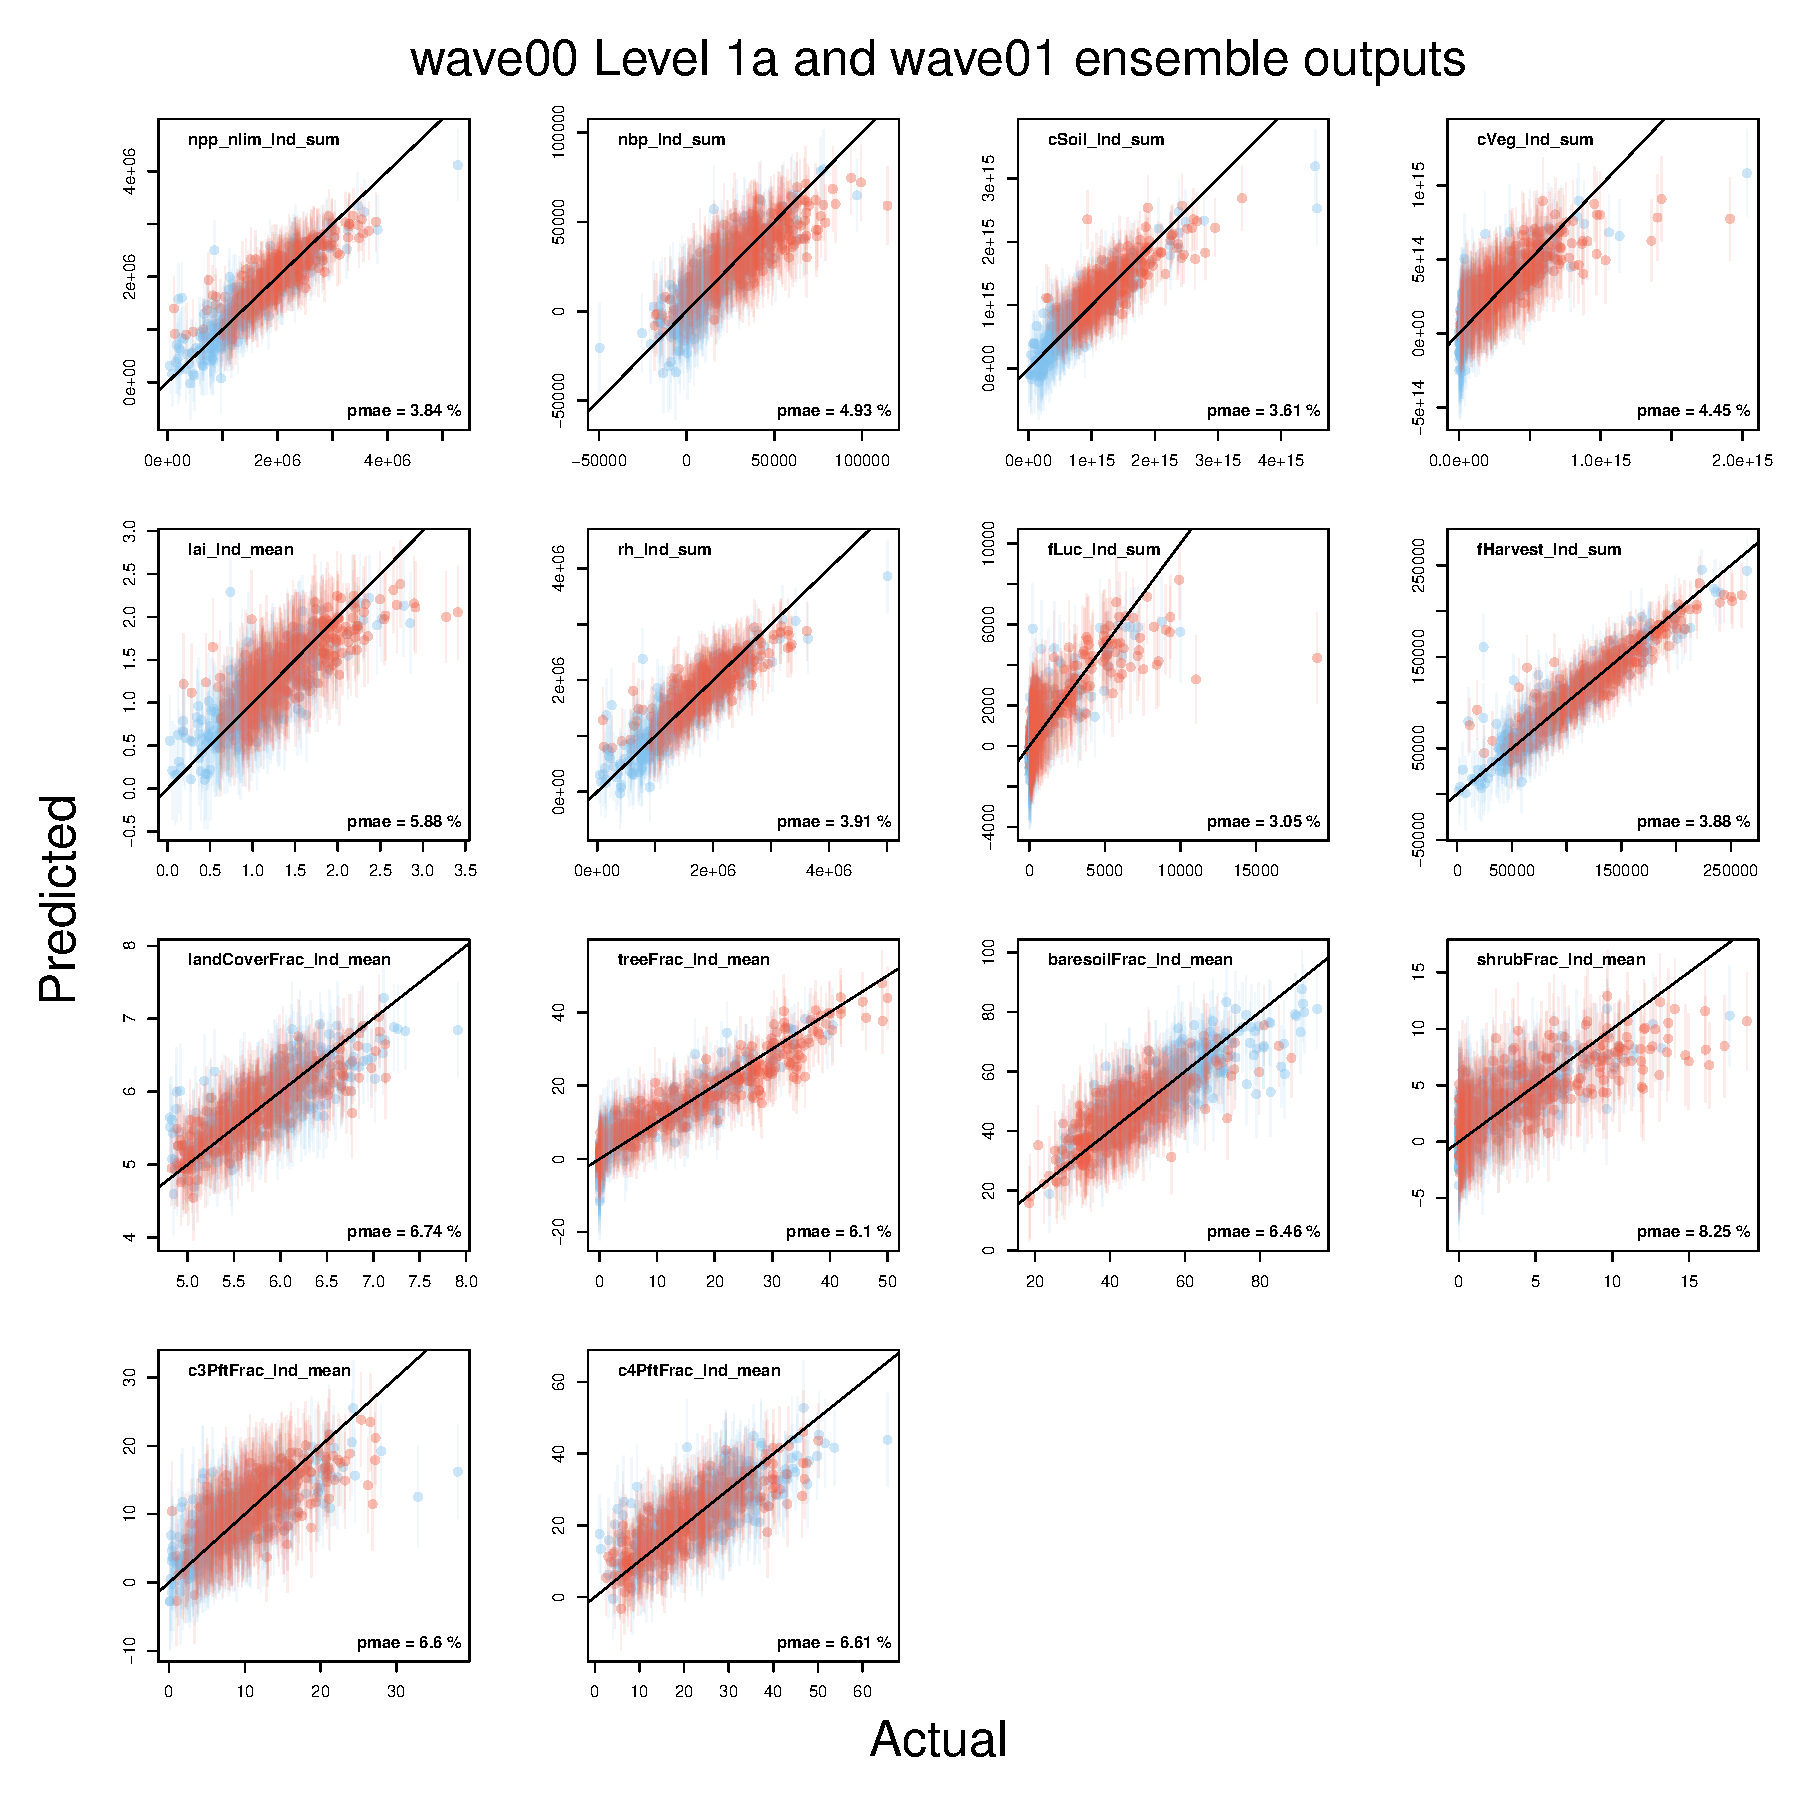
\includegraphics[width=12cm]{./figs/figA01.pdf}
\caption{Leave-one-out summaries of emulator fits for modern value carbon cycle quantities. First wave (wave00) is blue and the second wave (wave01) is red. }
\label{fig:kmloostats_Y_wave00_level1a_wave01}
\end{figure*}


%%% TWO-COLUMN FIGURES
%
%%f
\begin{figure*}[t]
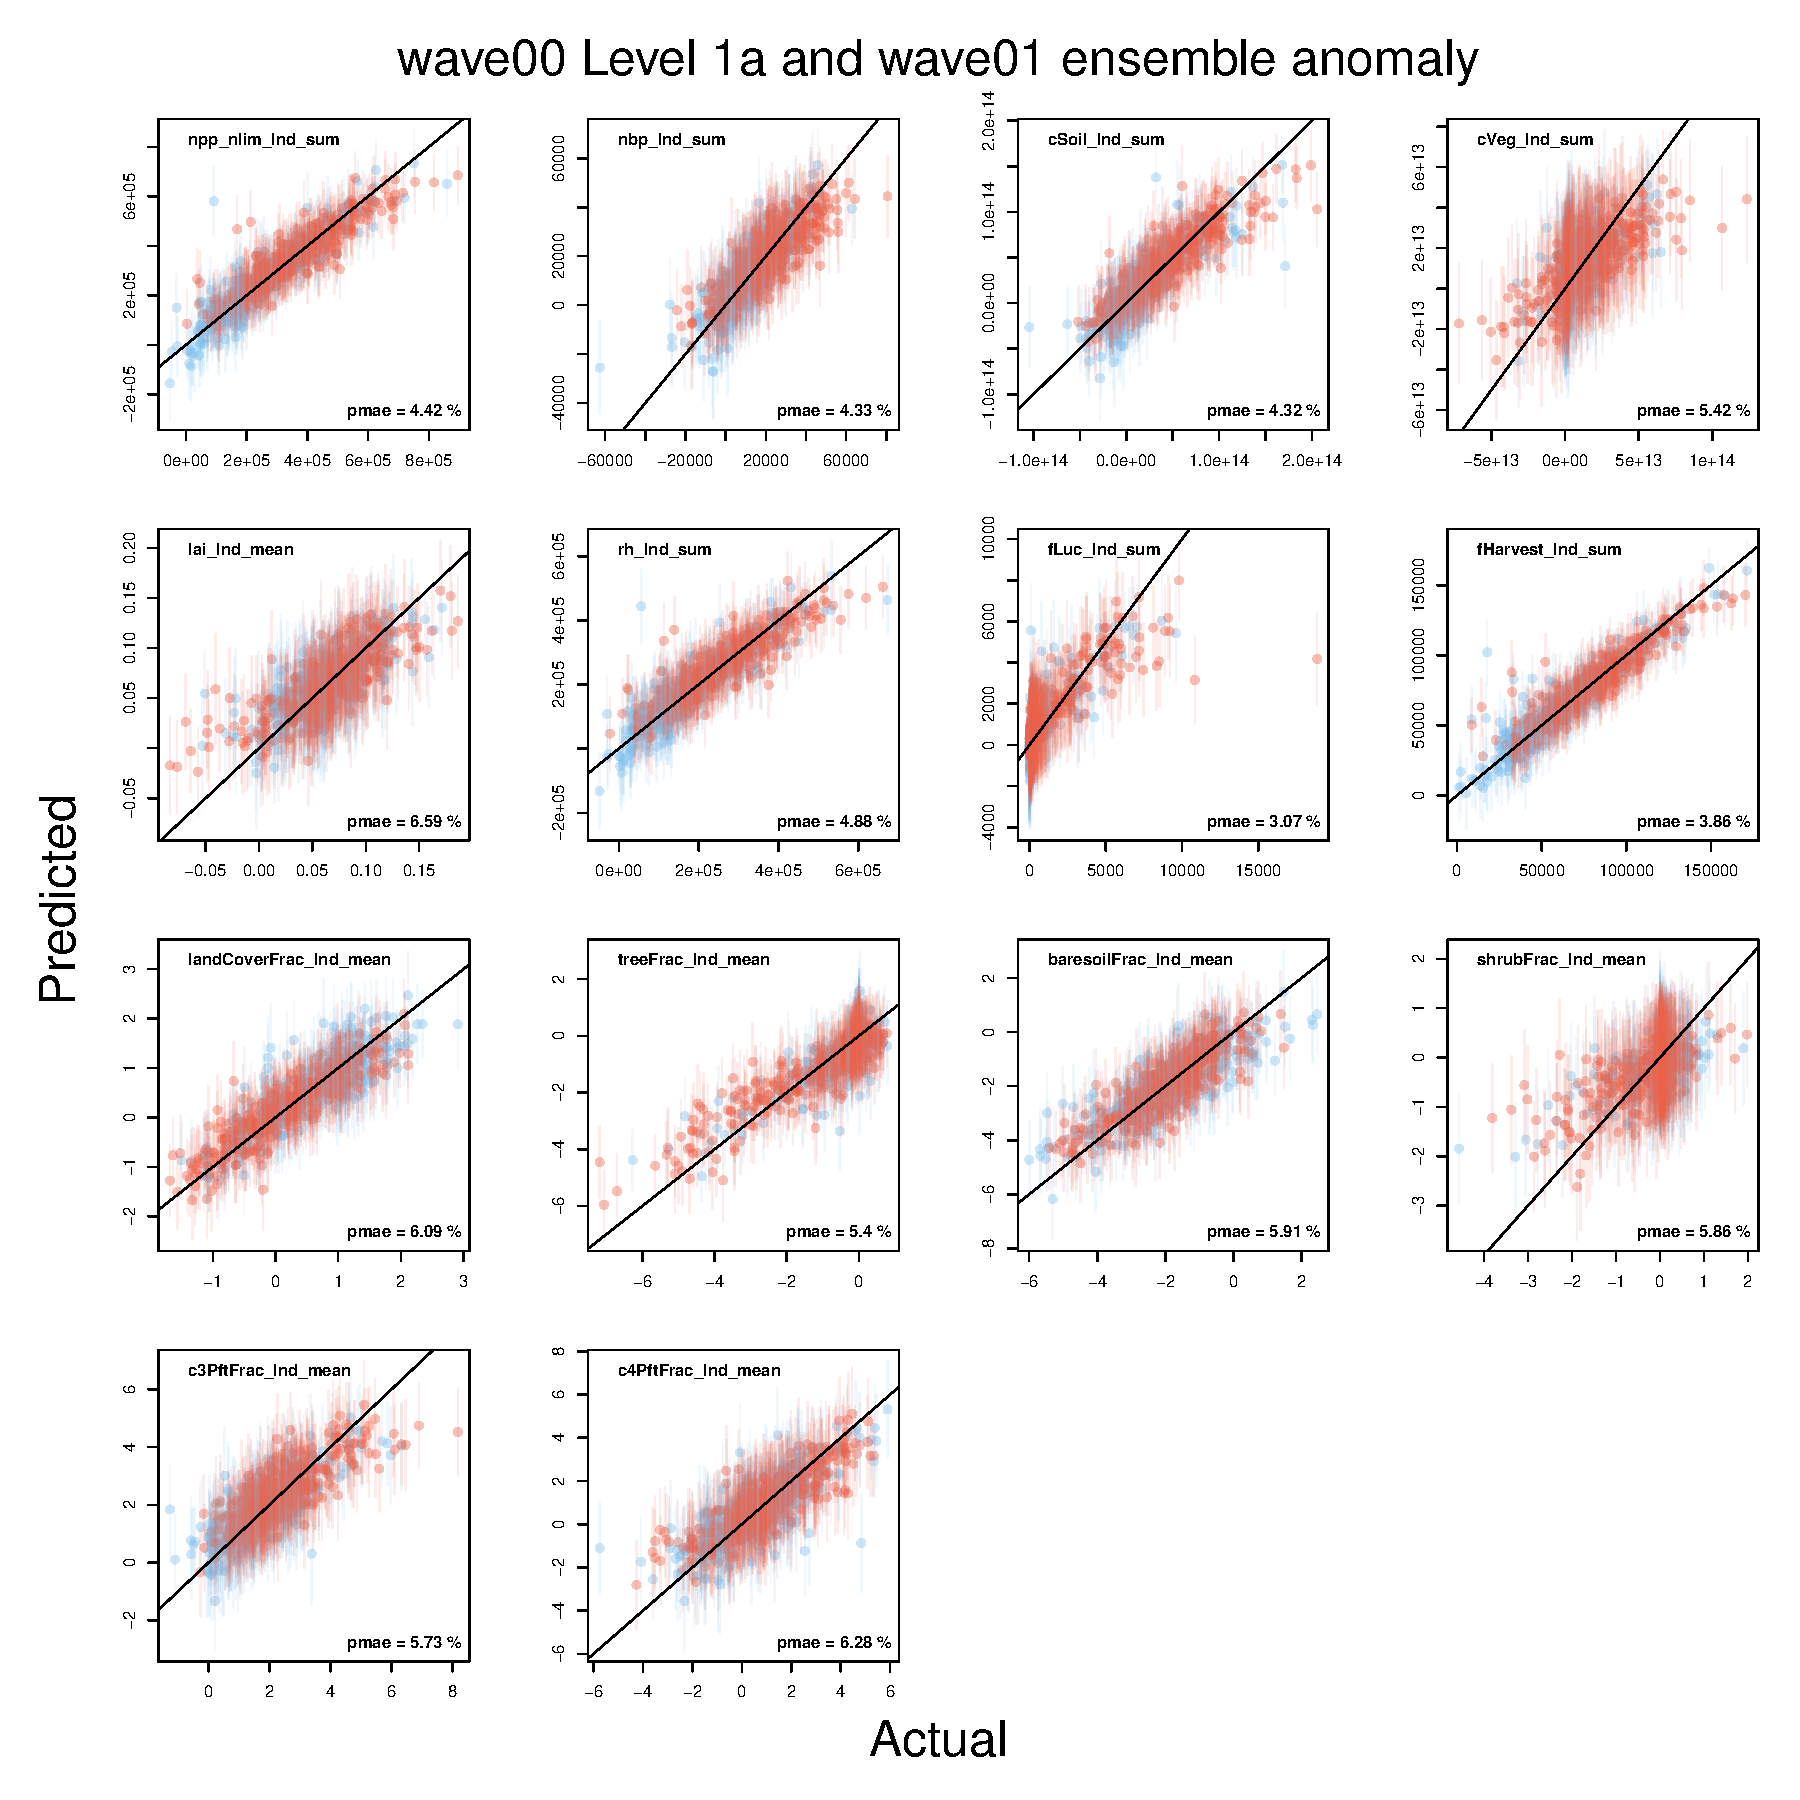
\includegraphics[width=12cm]{./figs/figA02.pdf}
\caption{Leave-one-out summaries of emulator fits for modern value anomaly carbon cycle quantities. First wave (wave00) is blue and the second wave (wave01) is red. }
\label{fig:kmloostats_YAnom_wave00_level1a_wave01}
\end{figure*}

%%% TWO-COLUMN FIGURES
%
%%f
\begin{figure*}[t]
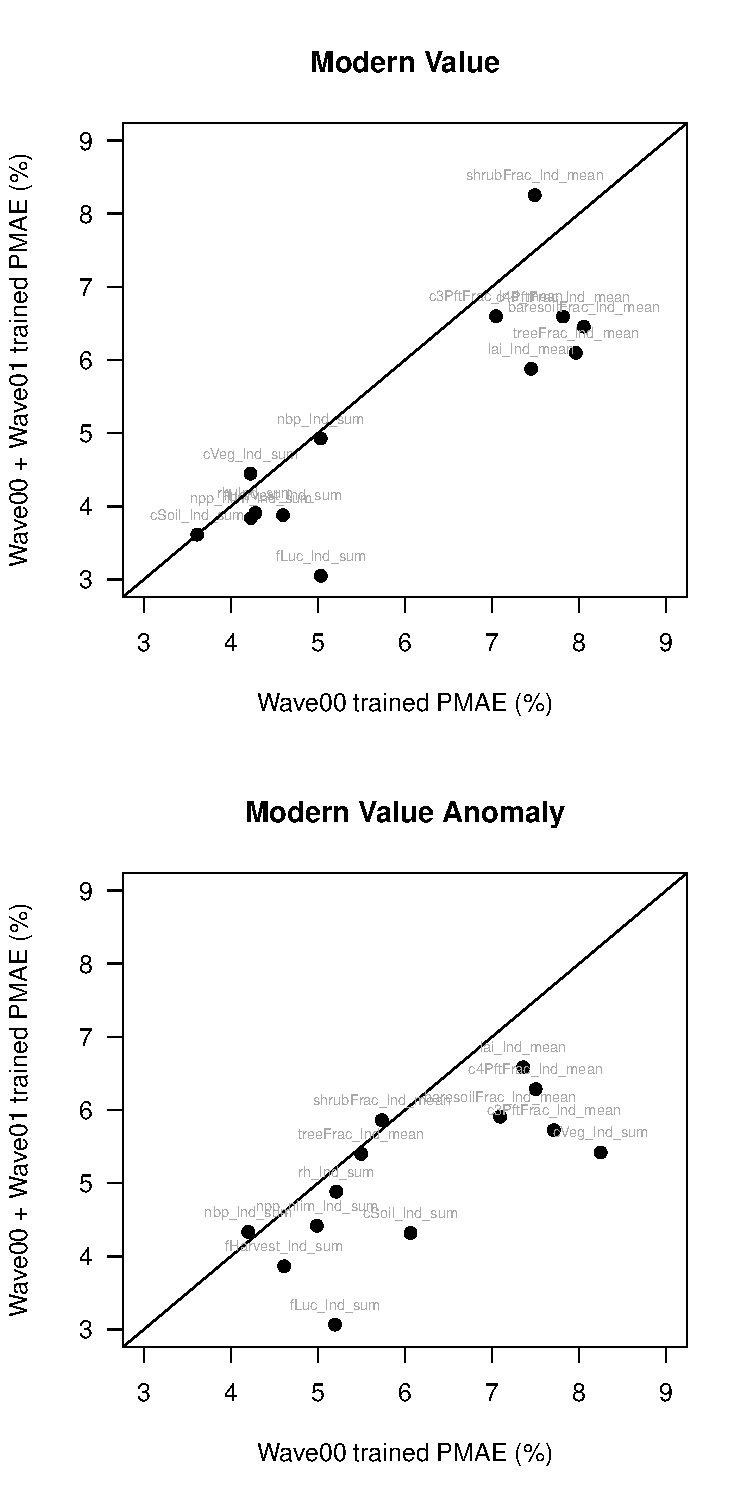
\includegraphics[width=6cm]{./figs/figA03.pdf}
\caption{Proportional mean absolute error (PMAE} summaries for selected JULES modern value (top) and anomaly (bottom) outputs. Horizontal axes show PMAE using only wave00 level 1a constrained outputs, while vertical axes show the same summary using wave00 and wave01 outputs. Outputs below the diagonal line show an overall improvement in emulator performance. 
\label{fig:PMAE_comparison}
\end{figure*}

\subsection{Predicting members that satisfy level 2 constraints}\label{app:level_2_pred} 

A useful measure of the practical utility of our emulator is the accuracy with which we can predict if a given input configuration will produce model output that conforms to a set of constraints. Here, we focus on the accuracy of our emulator for predicting ensemble members that conform to our reasonable "level2" constraints. These ensemble members produce output that is reasonable in a very broad way - roughly consistent with a functioning carbon cycle, our observations of the world, and the CMIP6 ensemble, but not directed at a particular set of observations.

We perform a Leave-one-out cross validation on the outputs that we use for the level2 constraint, namely the modern-day value of the global sum of NBP, NPP, soil carbon and vegetation carbon. We show the results of the leave-one-out posterior mean predictions in fig. \ref{fig:Y_const_loo}. If we treat the posterior mean predictions as model runs, and constrain them using the same thresholds as the level 2 results, we can convert them into a binary forecast for whether they are "in" or "out" of the constraint. While this loses some information, it is a useful summary. We predict 20 ensemble members correctly as "in" the constraints, and 311 correctly as "out". We predict 14 incorrectly as "out" when they should be "in" (false negative) and 17 incorrectly as "in" when they should be "out". A contingency table summarising these results is presented in \ref{table:level_2_contingency}. We use the R verification package \cite{R2015verification} to calculate a number of skill scores, including the Equitable Threat Score (ETS), which we calculate at 0.34, and the Heidike Skill Score (HSS), which we calculate at 0.51. These scores (as well as the raw numbers) indicate that we have a predictive system, which could well be improved.

\begin{table*}[t]
\caption{Confusion matrix for leave-one-out emulator predictions of whether the true model outputs conform to the level 2 output constraints}
\label{table:level_2_contingency}
\begin{tabular}{l l r r}
\tophline
 &  &  & Model \\ 
& & Out &  In\\
Emulator & Out & 309 &  14 \\
 & In & 14 & 24 \\

\bottomhline
\end{tabular}
\belowtable{} % Table Footnotes

\end{table*}

Studying fig. \ref{fig:Y_const_loo}, we see that a possible culprit for many of the constraint prediction errors is the relatively poor quality of the emulator for vegetation carbon (cVeg). That emulator predicts a relatively large number of ensemble members to have a lower vegetation carbon that we see in reality (and many close to zero), when the true vegetation is high. This leads to a number of "false negatives". Conversely, when the vegetation carbon is relatively low, there are a small number over-predicted, leading to false positives. This is not a consistent bias, so we cannot simply add a discrepancy value all across input space, more subtlety is required in order to improve the emulator and predictions.

We try a number of strategies to improve the emulator, including transformation of the cVeg output by taking logs, or square root. These can considerably improve the emulator for low values of the output. Unfortunately, we don't believe that the very low values are realisitic, and are therefore not very informative about higher values. Indeed, transforming the output has the impact of making the leave-one-out scores for the ensemble members that conform to level 2 constraints worse.

We try a number of different covariance types and optimisation methods within the emulator fitting process for cVeg, but none improves the performance for level 2 conforming ensemble members.

It appears that the initial design for the experiment was set too wide, with many ensemble members having unrealistically low carbon vegetation values. This meant that this emulator is difficult to build, output isn't smooth, and the constraint may well benefit from an iteration of the history matching, getting the initial ranges more close to being correct, and having smoother output.



\begin{figure*}[t]
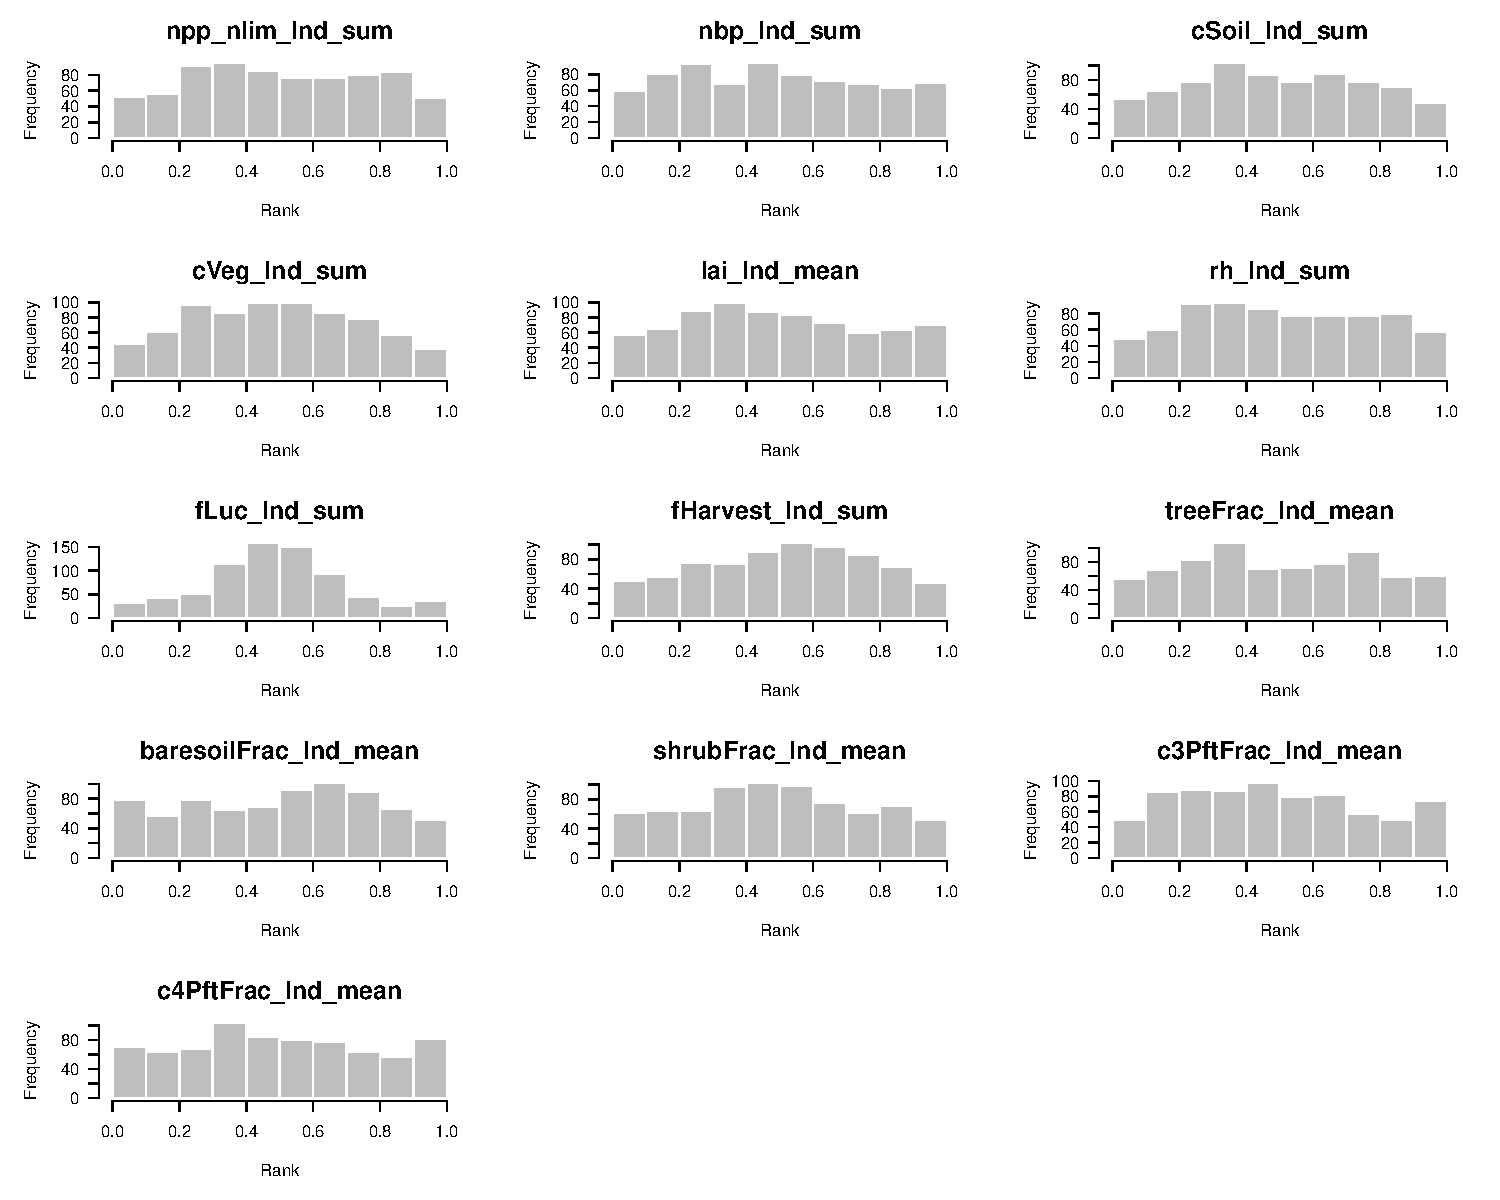
\includegraphics[width=12cm]{./figs/figA04.pdf}
\caption{Leave-one-out summaries }
\label{fig:Y_const_loo}
\end{figure*}

\section{FAST sensitivity analysis details}\label{app:sa_fast}

Summaries of FAST sensitivity analysis for both "modern value" and "anomaly" outputs of JULES-ES-1.0 can be found in fig. \ref{fig:FAST_sensmat_Y_level1a} and fig. \ref{fig:FAST_sensmat_YAnom_level1a} respectively.

\begin{figure*}[t]
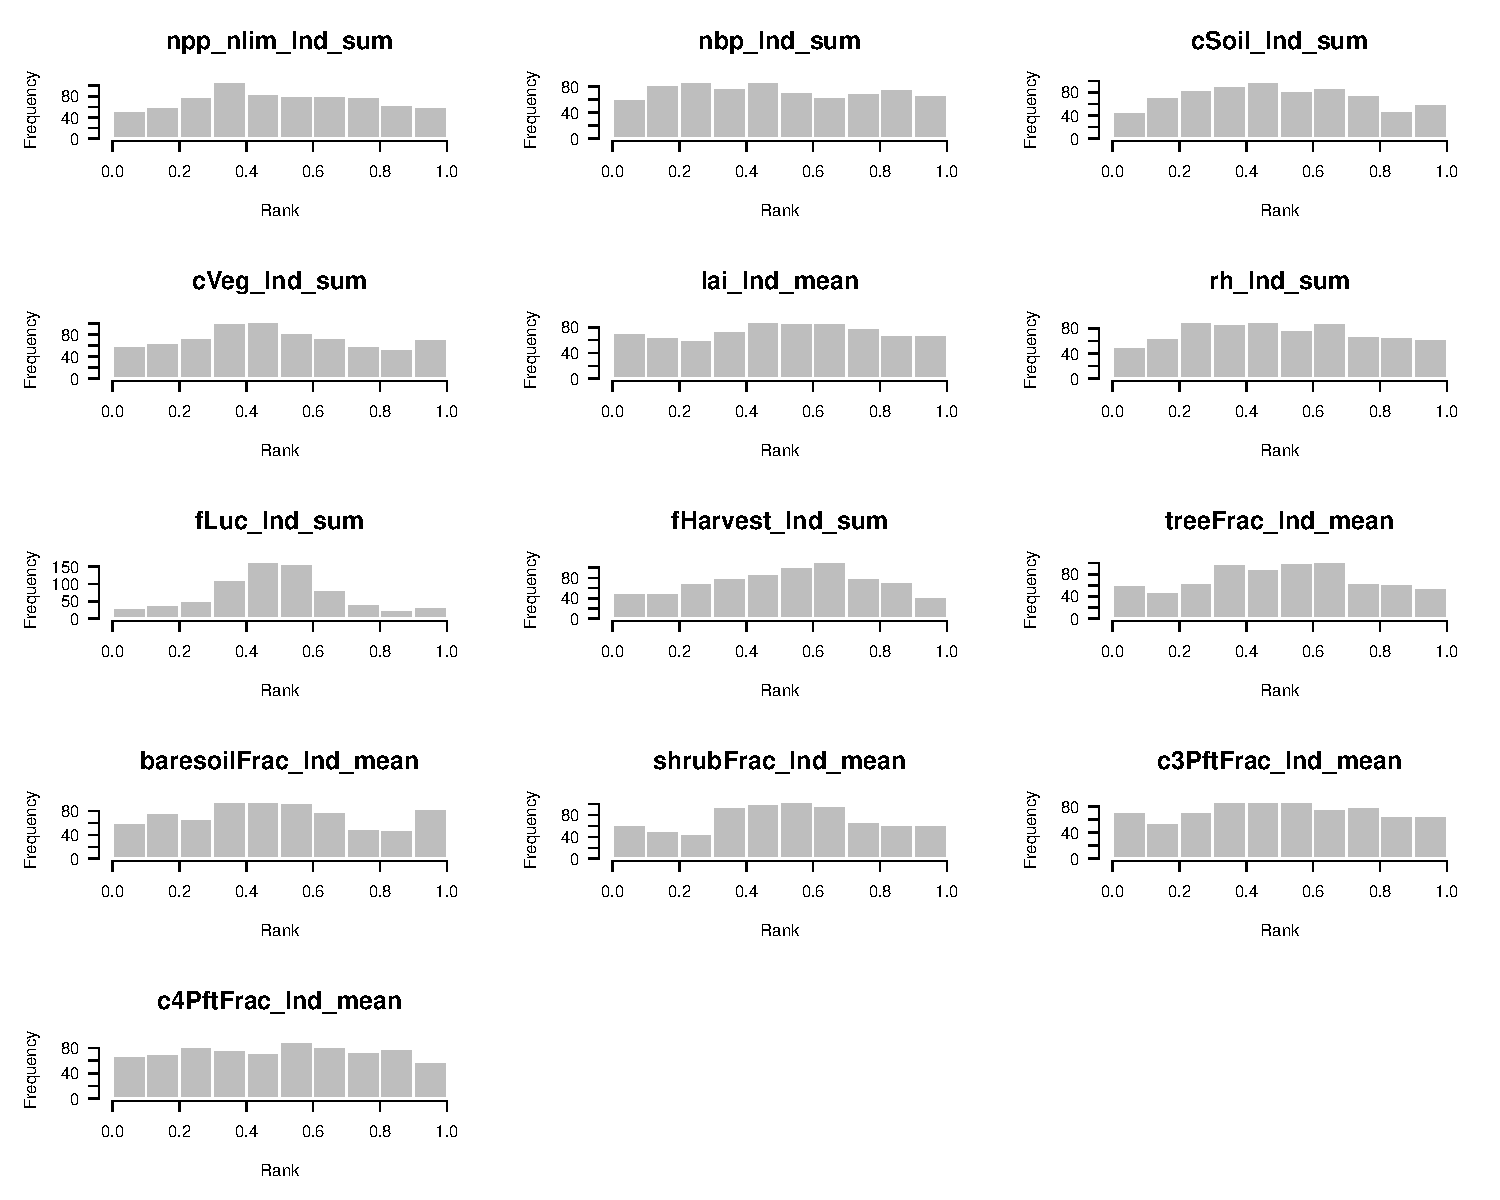
\includegraphics[width=12cm]{./figs/figA05.pdf}
\caption{FAST sensitivity analysis summary for modern value outputs.}
\label{fig:FAST_sensmat_Y_level1a}
\end{figure*}

\begin{figure*}[t]
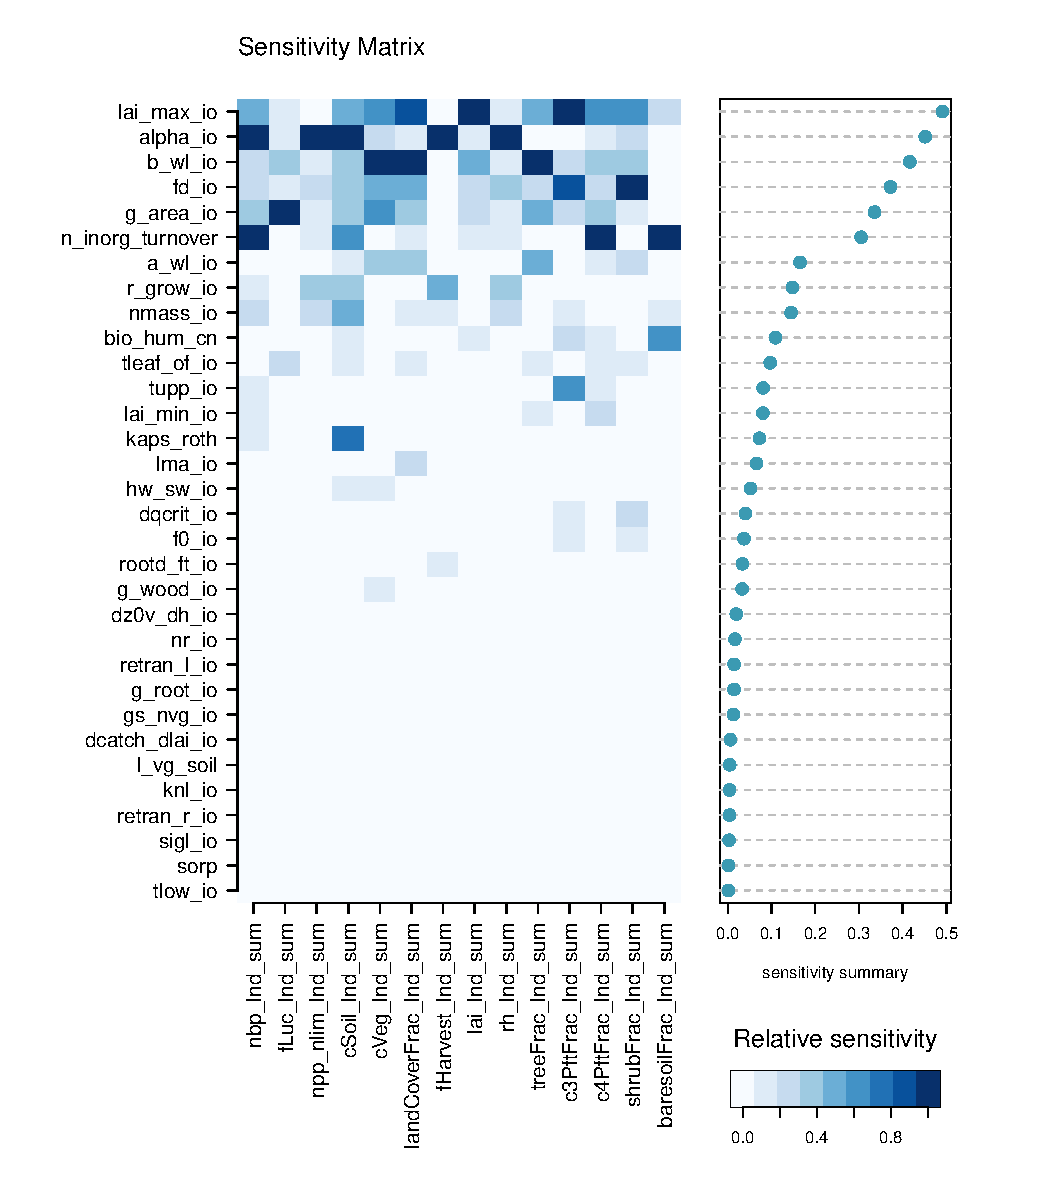
\includegraphics[width=12cm]{./figs/figA06.pdf}
\caption{FAST sensitivity analysis summary for anomaly outputs.}
\label{fig:FAST_sensmat_YAnom_level1a}
\end{figure*}



\noappendix       %% use this to mark the end of the appendix section. Otherwise the figures might be numbered incorrectly (e.g. 10 instead of 1).

%% Regarding figures and tables in appendices, the following two options are possible depending on your general handling of figures and tables in the manuscript environment:

%% Option 1: If you sorted all figures and tables into the sections of the text, please also sort the appendix figures and appendix tables into the respective appendix sections.
%% They will be correctly named automatically.

%% Option 2: If you put all figures after the reference list, please insert appendix tables and figures after the normal tables and figures.
%% To rename them correctly to A1, A2, etc., please add the following commands in front of them:

%\appendixfigures  %% needs to be added in front of appendix figures

%\appendixtables   %% needs to be added in front of appendix tables

%% Please add \clearpage between each table and/or figure. Further guidelines on figures and tables can be found below.

\authorcontribution{DM and AW planned the analysis. AW ran the simulations and the analysis was conducted by DM, with help from AW and ER. DM wrote the paper with contributions from AW and ER.} %% this section is mandatory

\competinginterests{The authors declare no competing interests.} 

%% this section is mandatory even if you declare that no competing interests are present

\begin{acknowledgements}

DM, ER and AW were supported by the Met Office Hadley Centre Climate Programme funded by BEIS, and by the Newton Fund through the Met Office Climate Science for Service Partnership Brazil (CSSP Brazil).

\end{acknowledgements}

%% REFERENCES

%% The reference list is compiled as follows:

%%\begin{thebibliography}{}

%%\bibitem[AUTHOR(YEAR)]{LABEL1}
%%REFERENCE 1

%%\bibitem[AUTHOR(YEAR)]{LABEL2}
%%REFERENCE 2

%%\end{thebibliography}

%% Since the Copernicus LaTeX package includes the BibTeX style file copernicus.bst,
%% authors experienced with BibTeX only have to include the following two lines:
%%
\bibliographystyle{copernicus}
 \bibliography{jules_ppe.bib}
%%
%% URLs and DOIs can be entered in your BibTeX file as:
%%
%% URL = {http://www.xyz.org/~jones/idx_g.htm}
%% DOI = {10.5194/xyz}


%% LITERATURE CITATIONS
%%
%% command                        & example result
%% \citet{jones90}|               & Jones et al. (1990)
%% \citep{jones90}|               & (Jones et al., 1990)
%% \citep{jones90,jones93}|       & (Jones et al., 1990, 1993)
%% \citep[p.~32]{jones90}|        & (Jones et al., 1990, p.~32)
%% \citep[e.g.,][]{jones90}|      & (e.g., Jones et al., 1990)
%% \citep[e.g.,][p.~32]{jones90}| & (e.g., Jones et al., 1990, p.~32)
%% \citeauthor{jones90}|          & Jones et al.
%% \citeyear{jones90}|            & 1990



%% FIGURES

%% When figures and tables are placed at the end of the MS (article in one-column style), please add \clearpage
%% between bibliography and first table and/or figure as well as between each table and/or figure.

% The figure files should be labelled correctly with Arabic numerals (e.g. fig01.jpg, fig02.png).


%% ONE-COLUMN FIGURES

%%f
%\begin{figure}[t]
%\includegraphics[width=8.3cm]{FILE NAME}
%\caption{TEXT}
%\end{figure}
%
%%% TWO-COLUMN FIGURES
%
%%f
%\begin{figure*}[t]
%\includegraphics[width=12cm]{FILE NAME}
%\caption{TEXT}
%\end{figure*}
%
%
%%% TABLES
%%%
%%% The different columns must be seperated with a & command and should
%%% end with \\ to identify the column brake.
%
%%% ONE-COLUMN TABLE
%
%%t
%\begin{table}[t]
%\caption{TEXT}
%\begin{tabular}{column = lcr}
%\tophline
%
%\middlehline
%
%\bottomhline
%\end{tabular}
%\belowtable{} % Table Footnotes
%\end{table}
%
%%% TWO-COLUMN TABLE
%
%%t
%\begin{table*}[t]
%\caption{TEXT}
%\begin{tabular}{column = lcr}
%\tophline
%
%\middlehline
%
%\bottomhline
%\end{tabular}
%\belowtable{} % Table Footnotes
%\end{table*}
%
%%% LANDSCAPE TABLE
%
%%t
%\begin{sidewaystable*}[t]
%\caption{TEXT}
%\begin{tabular}{column = lcr}
%\tophline
%
%\middlehline
%
%\bottomhline
%\end{tabular}
%\belowtable{} % Table Footnotes
%\end{sidewaystable*}
%
%
%%% MATHEMATICAL EXPRESSIONS
%
%%% All papers typeset by Copernicus Publications follow the math typesetting regulations
%%% given by the IUPAC Green Book (IUPAC: Quantities, Units and Symbols in Physical Chemistry,
%%% 2nd Edn., Blackwell Science, available at: http://old.iupac.org/publications/books/gbook/green_book_2ed.pdf, 1993).
%%%
%%% Physical quantities/variables are typeset in italic font (t for time, T for Temperature)
%%% Indices which are not defined are typeset in italic font (x, y, z, a, b, c)
%%% Items/objects which are defined are typeset in roman font (Car A, Car B)
%%% Descriptions/specifications which are defined by itself are typeset in roman font (abs, rel, ref, tot, net, ice)
%%% Abbreviations from 2 letters are typeset in roman font (RH, LAI)
%%% Vectors are identified in bold italic font using \vec{x}
%%% Matrices are identified in bold roman font
%%% Multiplication signs are typeset using the LaTeX commands \times (for vector products, grids, and exponential notations) or \cdot
%%% The character * should not be applied as mutliplication sign
%
%
%%% EQUATIONS
%
%%% Single-row equation
%
%\begin{equation}
%
%\end{equation}
%
%%% Multiline equation
%
%\begin{align}
%& 3 + 5 = 8\\
%& 3 + 5 = 8\\
%& 3 + 5 = 8
%\end{align}
%
%
%%% MATRICES
%
%\begin{matrix}
%x & y & z\\
%x & y & z\\
%x & y & z\\
%\end{matrix}
%
%
%%% ALGORITHM
%
%\begin{algorithm}
%\caption{...}
%\label{a1}
%\begin{algorithmic}
%...
%\end{algorithmic}
%\end{algorithm}
%
%
%%% CHEMICAL FORMULAS AND REACTIONS
%
%%% For formulas embedded in the text, please use \chem{}
%
%%% The reaction environment creates labels including the letter R, i.e. (R1), (R2), etc.
%
%\begin{reaction}
%%% \rightarrow should be used for normal (one-way) chemical reactions
%%% \rightleftharpoons should be used for equilibria
%%% \leftrightarrow should be used for resonance structures
%\end{reaction}
%
%
%%% PHYSICAL UNITS
%%%
%%% Please use \unit{} and apply the exponential notation


\end{document}
